\pdfoutput=1
\pdfcompresslevel=9
\pdfinfo
{
    /Author (Aleksy Barcz)
    /Title (Implementation aspects of graph neural networks)
    /Keywords (Graph neural networks, classification, graph processing, recursive neural networks)
}
%\documentclass[a4paper,polish,onecolumn,oneside,floatssmall,11pt,titleauthor,wide,openright]{mwrep}
%\usepackage[scale={0.7,0.8},paper=a4paper,twoside]{geometry}
\documentclass[a4paper,onecolumn,oneside,12pt,wide,floatssmall]{mwrep} % 11pt w szablonie, 12pt dla TimesNewRoman
\usepackage{amsmath}
\usepackage{amsfonts}
\usepackage{amssymb}
\usepackage{amsthm}
\usepackage{bookman}
\usepackage{bm}		% bold math symbols

\usepackage{geometry}
\usepackage[utf8x]{inputenc}
\usepackage[T1]{fontenc}
% \usepackage{t1enc}
% \usepackage[pdftex, bookmarks]{hyperref}
%\usepackage[pdftex, bookmarks=false]{hyperref}
\usepackage[pdftex, bookmarks=true, colorlinks=true,linkcolor=black,urlcolor=blue,citecolor=black]{hyperref}
%\def\url#1{{ \tt #1}}
\usepackage{url} % linki url w bibliografii
\usepackage{alltt}
\usepackage{booktabs} % eleganckie tabelki
\usepackage{mathtools} % wyrównane macierze, wymaga texlive-latex3
\usepackage{bm} % pogrubione greckie litery

\usepackage{listings}

\usepackage{pslatex} %Times New Roman

% marginesy
\textwidth\paperwidth
\advance\textwidth -55mm
\oddsidemargin-0.9in
\advance\oddsidemargin 33mm
\evensidemargin-0.9in
\advance\evensidemargin 33mm
\topmargin -1in
\advance\topmargin 13mm
\setlength\textheight{48\baselineskip}
\addtolength\textheight{\topskip}
\marginparwidth15mm

\clubpenalty=10000 % to kara za sierotki
\widowpenalty=10000 % nie pozostawia wdów
\brokenpenalty=10000 % nie dzieli wyrazów pomiędzy stronami
\sloppy

\tolerance4500
\pretolerance250
\hfuzz=1.5pt
\hbadness1450

\linespread{1.3}	% interlinia 1.5 linii

% dotfill with smaller dots
\makeatletter
\newcommand \Dotfill {\leavevmode \cleaders \hb@xt@ .25em{\hss .\hss }\hfill \kern \z@}
\makeatother

% ŻYWA PAGINA
\renewcommand{\chaptermark}[1]{\markboth{\scshape\small\bfseries \
#1}{\small\bfseries \ #1}}
\renewcommand{\sectionmark}[1]{\markboth{\scshape\small\bfseries\thesection.\
#1}{\small\bfseries\thesection.\ #1}}
\newcommand{\headrulewidth}{0.5pt}
\newcommand{\footrulewidth}{0.pt}
\pagestyle{uheadings}

\usepackage[pdftex]{color,graphicx}
\usepackage[english]{babel}
\usepackage[usenames,dvipsnames]{xcolor} % kolory dla listingow kodu

\usepackage{parcolumns}	% two-column paragraphs
\usepackage{subfigure}
\usepackage{floatrow}
% Table float box with bottom caption, box width adjusted to content
\newfloatcommand{capbtabbox}{table}[][\FBwidth]


% \textheight232mm
% \setlength{\textwidth}{\textwidth}
% \setlength{\oddsidemargin}{\evensidemargin}
% \setlength{\evensidemargin}{0.3cm}
\usepackage[sort, compress]{cite}

%\usepackage{multibib}
%\newcites{bk,st,doc,web}{Książki i~artykuły,Standardy i~zalecenia,Dokumentacja produktów,Publikacje i~serwisy internetowe}

\theoremstyle{definition}
\newtheorem{defn}{Definition}[section]
\newtheorem{exmp}{Example}[section]

\theoremstyle{plain}% default
\newtheorem{thm}{Theorem}[section]
\newtheorem{lem}[thm]{Lemma}
\newtheorem{prop}[thm]{Hipothesis}
\newtheorem*{cor}{Conclusion}

\theoremstyle{remark}
\newtheorem*{rem}{Remark}
\newtheorem*{note}{Remark}
\newtheorem{case}{Case}

\definecolor{ListingBackground}{rgb}{1,1,1}

\begin{document}

% kody źródłowe wplatane w tekst
\lstdefinestyle{incode}
{
basicstyle={\footnotesize},
keywordstyle={\bf\footnotesize\color{black}},
commentstyle={\em\footnotesize\color{gray}},
numbers=left,
stepnumber=5,
firstnumber=1,
numberfirstline=true,
numberblanklines=true,
numberstyle={\sf\tiny},
numbersep=10pt,
tabsize=2,
xleftmargin=17pt,
framexleftmargin=3pt,
framexbottommargin=2pt,
framextopmargin=2pt,
framexrightmargin=0pt,
showstringspaces=true,
backgroundcolor={\color{ListingBackground}},
extendedchars=true,
% title=\lstname,
captionpos=b,
% abovecaptionskip=1pt,
% belowcaptionskip=1pt,
frame=tb,
framerule=0pt,
breaklines=true,
}

% kody źródłowe z podpisem
\lstdefinestyle{outcode}
{
basicstyle={\footnotesize},
keywordstyle={\bf\footnotesize\color{black}},
commentstyle={\em\footnotesize\color{gray}},
numbers=left,
stepnumber=5,
firstnumber=1,
numberfirstline=true,
numberblanklines=true,
numberstyle={\sf\tiny},
numbersep=10pt,
tabsize=2,
xleftmargin=17pt,
framexleftmargin=3pt,
framexbottommargin=2pt,
framextopmargin=2pt,
framexrightmargin=0pt,
showstringspaces=true,
backgroundcolor={\color{ListingBackground}},
extendedchars=true,
% title=\lstname,
captionpos=b,
% abovecaptionskip=1pt,
% belowcaptionskip=1pt,
frame=tb,
framerule=0.1pt,
breaklines=true,
}

\pagenumbering{roman}
\renewcommand{\baselinestretch}{1.0}
\raggedbottom
%
\begin{titlepage}
    % Strona tytułowa
    \vbox to\textheight{\hyphenpenalty=10000
    \begin{center}
	\begin{tabular}{p{107mm} p{9cm}}
	    \begin{minipage}{9cm}
	      \begin{center}
	      Politechnika Warszawska \\
	      Wydział Elektroniki i~Technik Informacyjnych \\
	      Instytut Informatyki
	      \end{center}
	    \end{minipage}
	    &
	    \begin{minipage}{8cm}
	    \begin{flushleft}
	      Rok akademicki 2012/2013
	    \vspace*{2.75\baselineskip}
	    \end{flushleft}
	    \end{minipage} \\
	\end{tabular}
	\vspace*{2.5\baselineskip}
	\begin{center}
		
\includegraphics[height=3.5cm,width=3.5cm]{img/PW_logo.png}
	\end{center}
	\vspace*{2.2\baselineskip}{\Large \MakeUppercase{Praca dyplomowa magisterska}\par}
	\vspace{2\baselineskip}{\large Aleksy Stanisław Barcz\par}
	\vspace*{2\baselineskip}{\LARGE Implementation aspects of graph neural networks\par}

	\vspace*{7\baselineskip}
	\hfill\mbox{}\par\vspace*{\baselineskip}\noindent
	\begin{tabular}[b]{@{}p{3cm}@{\ }l@{}}
	    {\large\hfill } & {\large }
	\end{tabular}
	\hfill
	\begin{tabular}[b]{c}
		Opiekun pracy: \\
		{mgr inż. Zbigniew Szymański}
	\end{tabular}\par
	\vspace*{5\baselineskip}
    \begin{tabular}{p{\textwidth}}
    \begin{flushleft}
	\begin{minipage}{7cm}
	Ocena: \Dotfill
	\par\vspace{2.5\baselineskip}
	\Dotfill
	\vspace{0.5\baselineskip}
	\par\noindent
	\centerline{Podpis Przewodniczącego}
	\centerline{Komisji Egzaminu Dyplomowego}\par
	\end{minipage}
    \end{flushleft}
    \end{tabular}
    \end{center}}

    % Życiorys
    \newpage\thispagestyle{empty}
    \begin{tabular}{p{4cm} p{20cm}}
    \begin{minipage}{4cm}
    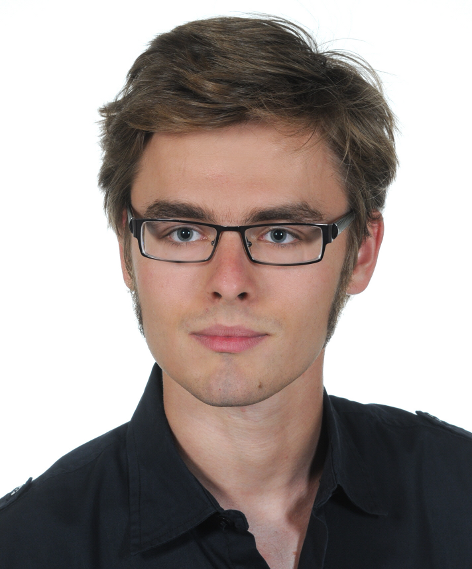
\includegraphics[height=4.8cm,width=4cm]{img/myphoto_cropped.png}
    \end{minipage}
    &
    \begin{minipage}{20cm}
    \begin{flushleft}
    \par\noindent\vspace{1\baselineskip}
    \begin{tabular}[h]{l l}
    {\normalsize Kierunek:} & Informatyka\\
    {\normalsize Specjalność:} & Inżynieria systemów informatycznych
    \end{tabular}
    \par\noindent\vspace{2\baselineskip}
    \begin{tabular}[h]{l r}
    {\normalsize Data urodzenia:} & {\normalsize 1988.01.28} \\
    {\normalsize Data rozpoczęcia studiów:} & {\normalsize 2012.02.20}
    \end{tabular}
    \par\noindent\vspace{2\baselineskip}
    \end{flushleft}
    \end{minipage}
    \end{tabular}
    \vspace*{1\baselineskip}
    \begin{center}
	{Życiorys}\par\bigskip
    \end{center}

    \noindent
	Ukończyłem XXVIII LO im. J.Kochanowskiego w Warszawie, w klasie o profilu matematyczno - informatycznym. Studia inżynierskie ukończyłem w lutym 2012 roku na kierunku Informatyka na Wydziale Elektroniki i Technik Informacyjnych Politechniki Warszawskiej. W trakcie studiów I i II stopnia brałem udział w wymianach studenckich programu Athens na Katholieke Universiteit Leuven \emph{(Fundamentals of artificial intelligence)} oraz w Télécom ParisTech \emph{(Emergence in complex systems)}.
    \par
    \vspace{2\baselineskip}
    \hfill\parbox{15em}{{\small\Dotfill}\\[-.3ex]
    \centerline{Podpis studenta}}\par
    \vspace{3\baselineskip}
 	{\noindent\MakeUppercase{Egzamin dyplomowy}} \par\bigskip\bigskip
    \par\noindent\vspace{1.5\baselineskip}
    Złożył egzamin dyplomowy w dniu \Dotfill 2013~r.
    \par\noindent\vspace{1.5\baselineskip}
    z wynikiem \Dotfill
    \par\noindent\vspace{1.5\baselineskip}
    Ogólny wynik studiów: \Dotfill
    \par\noindent\vspace{1.5\baselineskip}
    Dodatkowe wnioski i uwagi Komisji: \Dotfill
    \par\noindent\vspace{1.5\baselineskip}
    \Dotfill
    \par\noindent\vspace{1.5\baselineskip}
    \Dotfill

    % Streszczenie
    \newpage\thispagestyle{empty}
    \vspace*{2\baselineskip}
    \begin{center}
	{\large \MakeUppercase{Summary}}\par\bigskip
    \end{center}

    {\noindent
	This thesis describes the process of implementation of a Graph Neural Network, a classifier capable of classifying data represented as graphs. Parameters affecting the classifier efficiency and the learning process were identified and described. Implementation details affecting the classifier efficiency were described. Important similarities to other connectionist models used for graph processing were highlighted.
	}
    \vspace*{1\baselineskip}

    \noindent{Keywords}: {Graph neural networks, classification, graph processing, recursive neural networks}
    \par
    \vspace{4\baselineskip}

	\begin{center}
	\line(1,0){250}
	\end{center}

    \begin{center}
	{\large \MakeUppercase{ASPEKTY IMPLEMENTACYJNE GRAFOWYCH SIECI NEURONOWYCH}}\par\bigskip
    \end{center}
    {\noindent
	Praca stanowi raport z samodzielnej implementacji klasyfikatora typu Graph Neural Network (grafowa sieć neuronowa), pozwalającego na klasyfikację danych o strukturze grafowej. W ramach pracy zidentyfikowane zostały istotne dla klasyfikatora parametry, wpływające na przebieg procesu uczenia się klasyfikatora oraz na jakość uzyskanych wyników. Opisane zostały szczegóły implementacyjne klasyfikatora istotne dla jego działania. Klasyfikator został przedstawiony w kontekście podobnych rozwiązań w celu ukazania ścisłych powiązań między istniejącymi modelami przetwarzania danych o strukturze grafowej, opartymi na sieciach neuronowych.
	}
	
    \vspace*{1\baselineskip}

    \noindent{Słowa kluczowe}: {Grafowe sieci neuronowe, klasyfikacja, przetwarzanie grafów, rekursywne sieci neuronowe}

\end{titlepage}

% ex: set tabstop=4 shiftwidth=4 softtabstop=4 noexpandtab fileformat=unix filetype=tex spelllang=pl,en spell:


\begin{titlepage}
    % Strona tytułowa
    \vbox to\textheight{\hyphenpenalty=10000
    \begin{center}
	\begin{tabular}{p{107mm} p{9cm}}
	    \begin{minipage}{9cm}
	      \begin{center}
	      Politechnika Warszawska \\
	      Wydział Elektroniki i~Technik Informacyjnych \\
	      Instytut Informatyki
	      \end{center}
	    \end{minipage}
	    &
	    \begin{minipage}{8cm}
	    \begin{flushleft}
	      Rok akademicki 2012/2013
	    \vspace*{2.75\baselineskip}
	    \end{flushleft}
	    \end{minipage} \\
	\end{tabular}
	\vspace*{2.5\baselineskip}
	\begin{center}
		
\includegraphics[height=3.5cm,width=3.5cm]{img/PW_logo.png}
	\end{center}
	\vspace*{2.2\baselineskip}{\Large \MakeUppercase{Praca dyplomowa magisterska}\par}
	\vspace{2\baselineskip}{\large Aleksy Stanisław Barcz\par}
	\vspace*{2\baselineskip}{\LARGE Implementation aspects of graph neural networks\par}

	\vspace*{7\baselineskip}
	\hfill\mbox{}\par\vspace*{\baselineskip}\noindent
	\begin{tabular}[b]{@{}p{3cm}@{\ }l@{}}
	    {\large\hfill } & {\large }
	\end{tabular}
	\hfill
	\begin{tabular}[b]{c}
		Opiekun pracy: \\
		{mgr inż. Zbigniew Szymański}
	\end{tabular}\par
    \end{center}}

\end{titlepage}

% ex: set tabstop=4 shiftwidth=4 softtabstop=4 noexpandtab fileformat=unix filetype=tex spelllang=pl,en spell:


\tableofcontents
% \addcontentsline{toc}{chapter}{{Przedmowa1}{vii}}{vii}

%\setlength{\baselineskip}{7mm}
\newpage
\pagenumbering{arabic}
\setcounter{page}{1}


\chapter{Introduction}
The Graph Neural Network model is a connectionist classifier capable of classifying graphs. Most of the other existing neural network-based graph classifiers, such as RAAM~\cite{pollack1990recursive} or  LRAAM~\cite{sperduti1994labelling} and all solutions basing on them are capable of processing certain types of graphs only, in most cases DAGs (directed acyclic graphs) or DPAGs (directed positional acyclic graphs).
Several solutions were invented to deal with cyclic graphs, such as introducing a delay in the LRAAM encoding tree~\cite{goulon2005hopfield} or techniques mapping cyclic directed graphs to "recursive equivalent" trees~\cite{bianchini2003backpropagation}.
The problem of nonpositional graphs was also addressed by several authors, either by creating domain-specific encodings used to enforce a defined order on graph nodes~\cite{ivanciuc2003canonical} or by introducing various modifications to the classifier~\cite{bianchini2005recursive}.
However, most of the solutions dealing with cyclic and nonpositional graphs either complicate the classifier model, enlarge the input dataset or (in case of cycles) may result in information loss. The Graph Neural Network model can directly process most types of graphs, including cyclic, acyclic, directed, undirected, positional and nonpositional, which makes it a flexible solution.
There is a conceptual similarity between the GNN model and recursive neural networks~\cite{frasconi1998general}, however, the GNN model adapts a novel learning and backpropagation schema which simplifies processing different types of graphs.
This thesis describes the steps of implementation of a GNN classifier, including some details which were not described in the original article~\cite{scarselli2009graph}. The classifier was implemented in GNU Octave with two ideas in mind: providing a simple interface (similar to that of the Neural Networks toolbox) and maximum flexibility, that is the possibility of processing each kind of data that the theoretical model could deal with. The process of training a GNN and classification results were presented in detail. Listings of most important procedures were included in appendix~\ref{chap:code}.



\chapter{Domains of application}
This chapter presents domains where data is organized into a structured form, that is form of sequences or graphs. The necessity of processing differently such kinds of data arose from the structure of the data itself. To present this difference we must first summarize what is the task of classification and regression in the most common sense in data processing domain. A common statistical classifier (which later on is called a \emph{vectorial} classifier) takes as input \emph{samples} from a given \emph{dataset}, representing real world objects, and associates each sample with a category. The samples are fixed-length vectors of numeric values. Each position in such a vector represents a feature of the sample, which is quantified by a real or integer value. The mapping from features to positions in the vector is fixed and must hold for each sample in the dataset. The category is represented by a non-empty fixed-length vector of integer values, where once again the position of each value is meaningful (we can say it's a \emph{positional} representation). For the regression task, a vector of real (or integer) values is associated with each sample instead of a category. The domain of vectorial classifiers is well developed and includes, among other solutions, neural networks, support vector machines, naïve Bayes classifiers and random forests.

In the case of graph processing, the nature of the data is different. Each \emph{sample} is represented by a graph. A \emph{dataset} may consist of a single or several graphs. Each graph consists of nodes, connected with edges. Each node can be described by its \emph{label}, a fixed-length vector of reals. Each edge can also be labelled, with a fixed-length vector of reals of different size. Edges can be directed or undirected. An example of a simple graph was presented in Fig.~\ref{fig:simple_tree}.

\begin{figure}
\begin{center}
	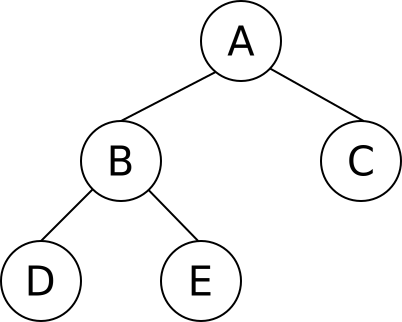
\includegraphics[scale=0.4]{img/tree}
	\caption{A simple binary tree}
	\label{fig:simple_tree}
\end{center}
\end{figure}

 If such a graph was to be used as input for a common classifier, it would be necessary to transform the structured representation into a plain vector. It could be accomplished in several ways, one of the most obvious would be to perform a preorder walk on the tree and list the node labels in the order they were visited. Such a walk would result in the representation $[A,B,D,E,C]$. It can be seen that the explicit information about node adjacency was lost. Instead, the information is provided implicitly, according to a coding which must be known a priori to properly interpret such a vector representation. That means that a model learning to classify such graph representations would have to learn the encoded relationship, instead of using it from the beginning to learn other, unknown and interesting relationships affecting the samples category. The resulting learning task becomes even harder if such sequential representations contain long-distance relationships. Different encodings from structured data to vectors exist, however, they all share that flaw.

Moreover, the inadequacy of simple vector representation becomes even more apparent when the graph structure becomes more complicated. First of all, if edge labels are present in the vector representation, the representation becomes a mix of data belonging to two different entities - nodes and edges. Once again the classifier doesn't know which part of the data corresponds to the first entity and which to the other. The same applies to directed and undirected edges. If two edges in a graph are connected by a directed edge, presumably one of the nodes in the relation has got a larger impact on the other than vice versa. On the contrary, an undirected or bidirectional edge edge implies an equal impact of both nodes on each other. What if a graph contains both types of edges? How should one type of edges be distinguished from the other one? Secondly, let's consider the case of cyclic dependencies. Even if a meaningful representation of the graph is built ignoring cycles, e.g. by constructing a minimum spanning tree, some explicit information about connections is lost. An example of such data are chemical compounds containing groups of atoms forming cyclic bonds. Another problem lies in the positional nature of vectorial data. If a representation is built by simply storing node labels one after another, this representation becomes vulnerable to any reordering of the children of a node. An additional effort must be made to assure a consistent ordering of the potentially difficult to order data, while the ordering of the children of a node may be irrelevant in the dataset considered.

It can be seen that in order to properly process structured data, a different approach must be used. The data should be processed in a way that exploits properly the information contained in its structure - by means of building a sufficient representation or by processing the structured data directly. Domains, where graph-oriented processing is already used include chemistry (QSAR, computer-aided drug design), pattern recognition and natural language processing.








\chapter{Graph processing models}
\noindent A model considered as fully capable of processing structured data, should be able to:
\begin{enumerate}
	\item build data representation
	\begin{enumerate}
		\item minimal
		\item exploiting sufficiently the structure of the data
		\item adequate for subsequent processing (classification, regression)
	\end{enumerate}
	\item perform classification / regression on the structured data
	\begin{enumerate}
		\item taking into consideration the structure encoded in the representation
		\item with a high generalization capacity
	\end{enumerate}
\end{enumerate}
These two main tasks are often intertwined with each other, as a classification procedure may affect the procedure of representation building and vice versa. It is also possible for a model to focus only on representation building, while leaving the task of processing to a common statistical classifier, such as a support vector machine. Two main families of models capable of processing structured data are the \emph{symbolic} and the \emph{connectionist} family. The first one originates in the artificial intelligence domain and focus on inferring relationships by means of inductive logic programming. The \emph{connectionist} models focus on modelling relationships with the use of interconnected networks of simple units. The different models originating from these two families are:
\begin{enumerate}
	\item inductive logic programming
	\item evolutionary algorithms
	\item probabilistic models: Bayes networks and Markov random fields
	\item graph kernels
	\item neural network models
\end{enumerate}
The main area of interest of this thesis are the connectionist models based on neural networks. The connectionist models make the fewest assumptions about the domain of the dataset and thus provide a potentially most general method for processing structured data.


\chapter{History}
This chapter summarizes the history of connectionist models used for graph processing. All these models originate from the feed-forward neural networks (FNNs). The history of neural networks begins in 1943 with the McCulloch–Pitts (MCP) neuron model, following with the Rosenblatt perceptron classifier in 1957. The feed-forward neural network model was developed during the following three decades and a conclusive state was reached in all major fields of related research until approximately 1988. The FNN model reached maturity in its field of application: classification and regression performed on unstructured positional samples of fixed size. In the '80s a new branch of the neural networks family began to develop - the recurrent neural networks (RNN). The RNN model is capable of processing sequences of varying length (potentially infinite), which makes them suitable for dealing with time-varying sequences or biological samples of various length~\cite{saha2006prediction}. However, a slightly different model had to be invented to properly process graph data.

\section{Hopfield networks}
One of the earliest attempts to classify structured data with neural networks was using the Hopfield networks~\cite{goulon2005hopfield}. A common application of a Hopfield network is an auto-associative memory, which learns to reproduce patterns provided as its inputs. (The task to be learned is the mapping $\bm{x}_i \Rightarrow \bm{x}_i$, where $\bm{x}_i$ is a pattern of fixed size $n$.) Afterwards, when a new sample is presented to the trained network, the network associates it with the most similar pattern it had learned. Subsequently, it was discovered, that by using a Hopfield network to reproduce a predefined successor of a pattern instead of the pattern itself, the network can be used as an hetero-associative memory, capable of reproducing sequences of patterns ($\bm{x}_i \Rightarrow \bm{x_{i+1}}$). The next step towards graph processing was to use Hopfield networks to learn the task of reproducing \emph{all} the successors (or predecessors) of a node, that is to learn the mapping $\bm{x}_i \Rightarrow succ[\bm{x}_i]$, where $x_i$ is the $i$th node label and $succ[\bm{x}_i]$ denotes a vector obtained by stacking together the labels of all the successors of node $\bm{x}_i$, one after another. For such task the maximum outdegree of a node (the maximum number of its successors) has to be known prior to the network training. $NIL$ patterns are used as extra successors labels whenever a considered node $\bm{x}_i$ has an outdegree smaller than the maximum value chosen. The last and somehow different application of Hopfield networks was to use a Hopfield network once again as an auto-associative memory, used for retrieving whole graphs. In such case the graph adjacency matrices ($N \times N$) are encoded into a network having $N(N - 1)/2$ neurons~\cite{goulon2005hopfield}, where $N$ is the number of nodes in a graph. To obtain an adequate generalisation, graphs isomorphic to the training set are generated and fed to the network~\cite{kree1988recognition}.

\section{RAAM}
The Recursive Auto-Associative Memory (RAAM) was introduced by Pollack in 1990~\cite{pollack1990recursive}. The RAAM model is a generalisation of the Hopfield network model~\cite{goulon2005hopfield}, providing means to meaningfully encode directed positional acyclic graphs (DPAGs). A distinctive feature of the RAAM model is that is can be used to encode graphs with labeled terminal nodes only. (The terminal nodes are nodes with outdegree equal to zero, that is nodes having no children. In the case of trees, leaves are terminal nodes.) That is, no node other than the terminal nodes of a graph may be labelled. No edge labels are permitted. The most straightforward domain of application for the RAAM model is thus natural language processing, where sentences can be decomposed to syntax graphs.\\
\noindent The RAAM model is capable of:
\begin{itemize}
	\item building compressed representation of structured data
	\item building meaningful representation: similar samples are represented in a similar way
	\item constrained generalisation: representing data absent in the training set
\end{itemize}
The RAAM model is composed of two units: \emph{compressor} and \emph{reconstructor}. Together they form a three-layer feed-forward neural network which works as an auto-associative memory. The \emph{compressor} is a fully connected two-layer neural network with $n$ input lines and $m$ output neurons. The number of output neurons, $m$ determines the size of a single encoded node representation. The number of input lines, $n$ must be a multiple of $m$, such that $n = k \cdot m$, where $k$ is the maximum outdegree of a node in the considered graphs. For each terminal node its representation consists of its original label. For each non-terminal node $i$ its representation, $\bm{x}_i$ is built by feeding the compressor with encoded representation of the $i$th nodes children.

To assure that the compressed representation is accurate and lossless, it is fed to the \emph{reconstructor}. The reconstructor is also a fully connected two-layer neural network, however it has $m$ input lines and $n$ output neurons. It is fed with compressed representations of nodes and is expected to produce the original data that was fed to the compressor. This procedure is repeated for all non-terminal nodes of a graph, until all encoded representations can be accurately decoded into original data. More precisely, the representation $\bm{x}_i$ of the $i$th node of the graph is given by Eq.~\ref{eq:raam_representation}, where $f$ denotes the function implemented by the compressor unit, $\bm{l}_i$ - the label of $i$th node, $\bm{x}_{ch[i]}$ - a vector obtained by stacking representations of all children of $i$th node one after another, $k$ - the maximum outdegree of a node in the graph.

\begin{equation}
\bm{x}_i = \left\{
\begin{array}{l l}
	\bm{l}_i & \quad \text{if $i$ is terminal} \\
	f(\bm{x}_{ch[i]}) & \quad \text{otherwise}
\end{array}
\right.
\label{eq:raam_representation}
\end{equation}

\noindent A sample graph that can be encoded using the RAAM model is presented in Fig.~\ref{fig:tree_for_raam}. The non-terminal nodes are enumerated for convenience only (only terminal nodes are labelled).

\begin{figure}
\begin{center}
	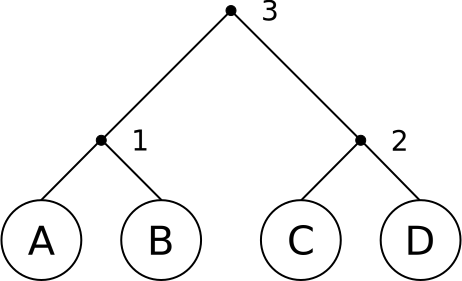
\includegraphics[scale=0.4]{img/tree_for_raam}
	\caption{A sample graph that can be processed using RAAM}
	\label{fig:tree_for_raam}
\end{center}
\end{figure}

\begin{figure}
\begin{center}
	
\includegraphics[scale=0.4]{img/raam1-3}
	\caption{Training set for the example graph}
	\label{fig:raam1-3}
\end{center}
\end{figure}

To encode the sample graph, the representations of nodes $1$ and $2$ must be built first. The representation of node $1$ is built by feeding the pair of labels $(A, B)$ to the compressor which encodes them into the representation $\bm{x}_1$. The representation $\bm{x}_1$ is then fed to the reconstructor, which produces a pair of labels $(A', B')$. If the resulting labels $A'$ and $B'$ are not similar enough to the original labels $A$ and $B$, the error is backpropagated through the compressor-reconstructor three-layer network. Similarly, the pair $(C, D)$ is processed by the same compressor-reconstructor pair and compressed into the representation $\bm{x}_2$. Then, the pair $(\bm{x}_1, \bm{x}_2)$ is once again fed to the compressor, which produces $\bm{x}_3$, the representation of the root node. This is also the compressed representation of the whole graph, from which the whole graph can be reconstructed by using the reconstructor unit. The training set, consisting of three label pairs, is presented in~Fig.~\ref{fig:raam1-3}. The light grey areas denote the compressor network, while the dark grey areas denote the reconstructor. Such a training set (or a larger one if the dataset consists of more than one graph) must be repeatedly processed by the RAAM model in the training phase. When the model is trained, the compression of the whole graph occurs as presented in~Fig.~\ref{fig:raam_compression}. Reconstruction of the graph is presented in~Fig.~\ref{fig:raam_reconstruction}. It is worth mentioning that a trained RAAM model can be used to process graphs with different structures.

\begin{figure}
\begin{center}
	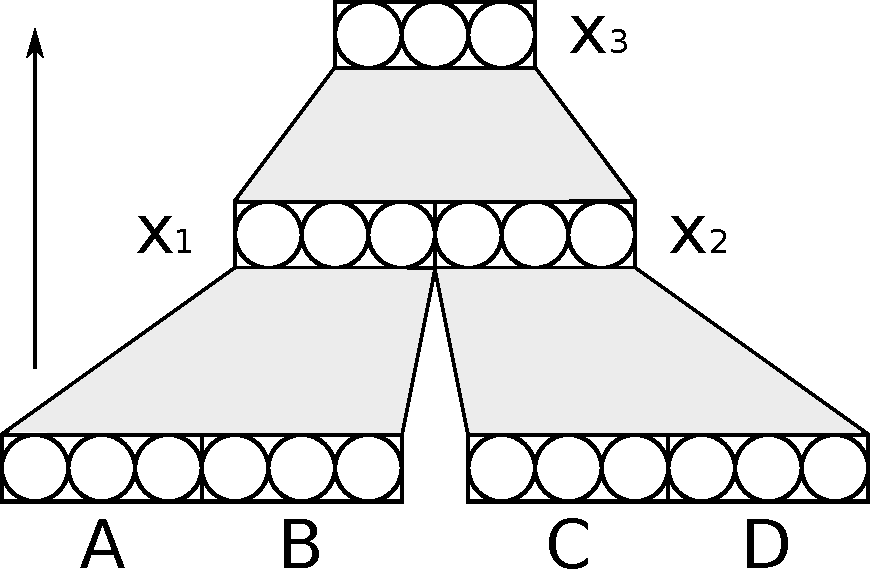
\includegraphics[scale=0.4]{img/raam_encode}
	\caption{Graph compression using trained RAAM model}
	\label{fig:raam_compression}
\end{center}
\end{figure}

\begin{figure}
\begin{center}
	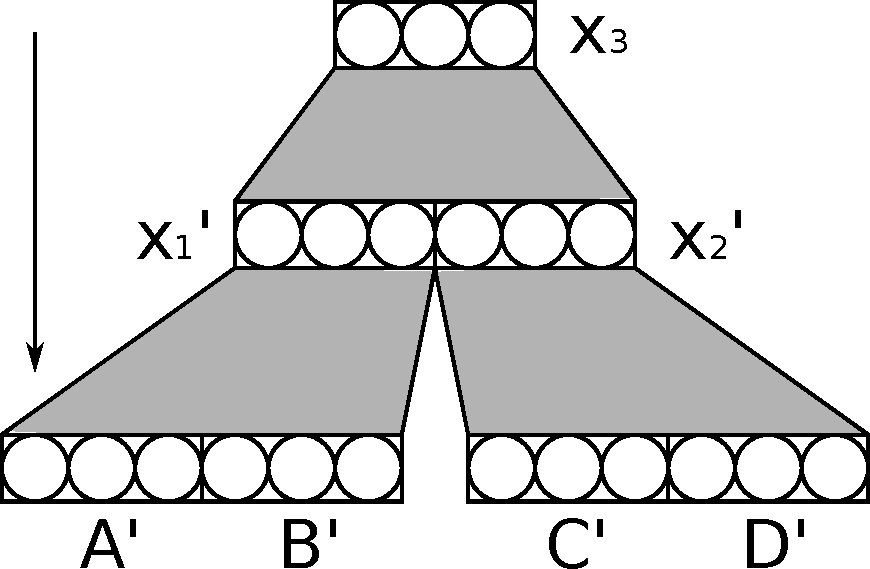
\includegraphics[scale=0.4]{img/raam_decode}
	\caption{Graph reconstruction from $\bm{x}_3$ using trained RAAM model}
	\label{fig:raam_reconstruction}
\end{center}
\end{figure}

A significant feature of the RAAM model is that a small reconstruction error in the case of non-terminal nodes may render the reconstruction of terminal nodes impossible. Therefore in the process of training a RAAM classifier it is necessary to set the acceptable reconstruction error value much smaller for the non-terminal nodes than for the terminal ones.

A major drawback of the RAAM model is the \emph{moving target} problem. That is, a part of the learning set (the representations $\bm{x}_1$ and $\bm{x}_2$ from the example) changes during training. In such a case the training phase may not converge to an acceptable state~\cite{goulon2005hopfield}. However, a different training schema is possible, based on the BPTS algorithm~\cite{goulon2005hopfield}. (An extensive description of the BPTS algorithm, \emph{encoding networks}, and the \emph{shared weights} technique is provided in the following chapters.) An encoding network is built out of identical instances of the compressor and reconstructor units (Fig.~\ref{fig:raam_tree}), with structure reflecting the structure of the processed graph (if the dataset consists of multiple graphs, such procedure is repeated for every graph in the dataset). All instances of the compressor unit share their weights and all instances of the reconstructor unit share their weights - which is called the \emph{shared weights} technique. The labels of terminal nodes are fed to the processing network and the resulting error can be backpropagated from the last layer using the Backpropagation Through Structure~\cite{kuchler1996inductive} algorithm (BPTS). It is worth mentioning, that the authors of such modified RAAM model propose using an additional layer of hidden neurons in the compressor and reconstructor units. In such case the light grey and dark grey areas on the figures would denote not only neuron connections between two layers, but also an additional hidden layer. Such modification allows to partially separate the problem of the data model complexity (i.e. how complex should the RAAM model be to properly compress the data) from the size of terminal node labels which affects directly the number of input lines to the compressor unit and thus the compressed representation size.

\begin{figure}
\begin{center}
	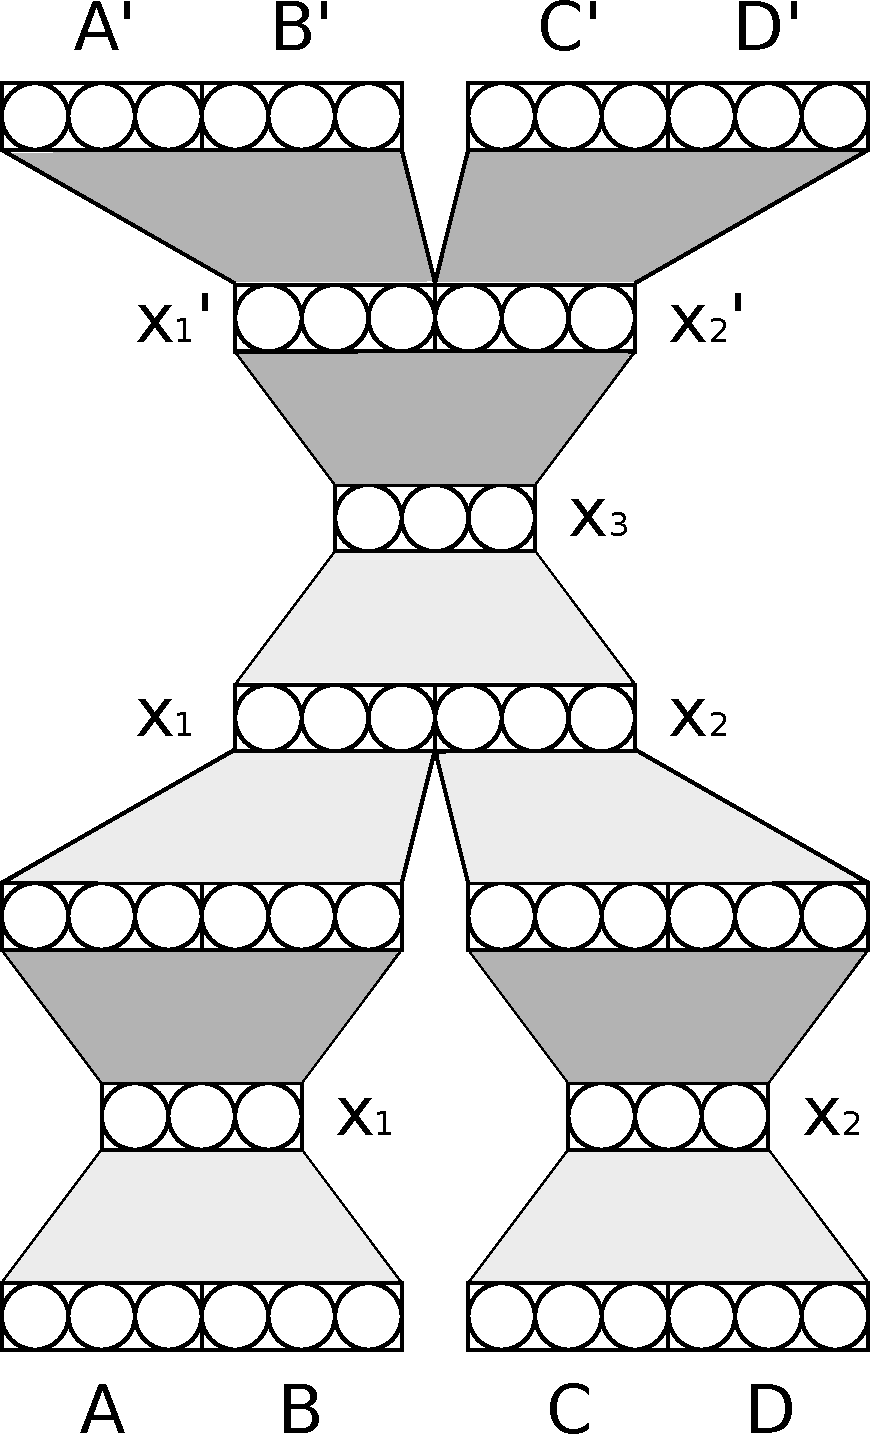
\includegraphics[scale=0.4]{img/raam_tree}
	\caption{Training RAAM using the BPTS procedure}
	\label{fig:raam_tree}
\end{center}
\end{figure}

The most important parameter of the RAAM model is the size of the compressed representation. On one hand, the size should be large enough to contain all the necessary compressed information about the encoded graph. On the other hand, it should be small enough for the compression mechanism to build a minimal representation, which stores only the necessary information about the dataset. If the size is too large, the trained model would store redundant information, memorizing the training set. This would result in a poor ability to process unseen data. Experiments with natural language syntax processing~\cite{pollack1990recursive} proved that when the size of the compressed representation is accurate for the problem, the RAAM model is showing some constrained generalisation properties. That is, unseen data with structure similar to the training set was processed properly by the trained RAAM model.

A drawback of the standard RAAM model is the termination problem. The reconstructor can't distinguish between terminal representations (node labels) and compressed representations, which should be further reconstructed. To solve this problem, an additional encoding neuron can be introduced (increasing the representation size by one), which takes a different value for terminal and non-terminal representations~\cite{stolcke1992tree}.

\section{LRAAM}
The most important constraint of the RAAM model is the fact that only terminal nodes of the processed graphs (DPAGs) can contain labels. This problem was addressed by the Labeling RAAM model~\cite{sperduti1994labelling} (LRAAM, 1994), which separated the concepts of node labels and node representations. In the RAAM model the terminal nodes are represented by their labels. The LRAAM model introduced the concept of \emph{pointers}, which was used to describe a node representation which has to be learnt, regardless of whether the node is terminal or not. The pointers are built by compressor units (FNN with two or more layers) and they are decoded into graph structure by reconstructor units. More precisely, the pointer to $i$th node of the graph is calculated according to Eq.~\ref{eq:lraam_pointer}, where $\bm{x}_i$ stands for pointer to the $i$th node, $f$ is the function implemented by the compressor unit, $\bm{l}_i$ is the $i$th node label, $\bm{x}_{ch[i]}$ is a vector obtained by stacking pointers to all children of $i$th node one after another and $k$ is the maximum outdegree of a node in the considered graph.

\begin{equation}
\bm{x}_i = f(\bm{l}_i, \; \bm{x}_{ch[i]})
\label{eq:lraam_pointer}
\end{equation}

Whenever a node outdegree is smaller than $k$ (especially in the case of terminal nodes), the missing child pointers are substituted by the $NIL$ pointer, a special value representing the lack of node. The value of the node label is stacked together with all the child pointers values to form an input vector which is fed to the compressor unit. The number of output neurons of the compressor unit (the size of a pointer $\bm{x}_i$) is $m$. Let's denote the size of the label $\bm{l}_i$ by $p$. The compressor unit must have $n = p + k \cdot m$ input lines which is also the number of reconstructor unit output neurons. The possibility of describing each graph node with its label provides a simple solution to the termination problem~\cite{sperduti1994labelling}. An additional value can be appended to each label, stating if the node is a terminal node or not. By using this method no change in the LRAAM model is needed.

Just like the RAAM model, the LRAAM model experience the problem of the \emph{moving target}. The same technique of \emph{shared weights} can be applied~\cite{goulon2005hopfield}, which results in building a large encoding network composed of identical units. A sample graph and the encoding network obtained by cloning the compressor and reconstructor units to reflect the sample graph structure are presented in Fig.~\ref{fig:lraam_tree}. As $A$ and $B$ are terminal nodes, their labels are fed to the compressor unit altogether with $NIL$ pointers representing the missing nodes. Then the compressed representation $\bm{x}_{A}$ is built for node $A$ and the compressed representation $\bm{x}_{B}$ is built for node $B$. The representations $\bm{x}_A$ and $\bm{x}_B$ are then fed altogether with the label $C$ to the compressor, to build the representation $\bm{x}_C$ of node $C$, which is also the compressed representation of the whole graph.

\begin{figure}
\begin{center}
	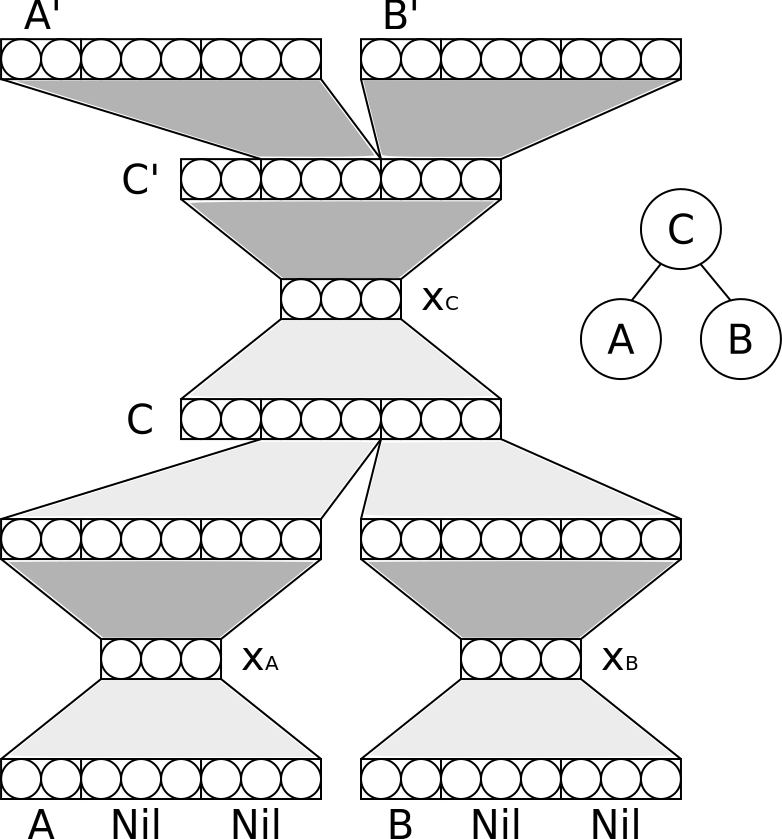
\includegraphics[scale=0.4]{img/lraam_tree}
	\caption{LRAAM encoding tree for the graph shown}
	\label{fig:lraam_tree}
\end{center}
\end{figure}

An extension of the LRAAM model exists for cyclic graphs~\cite{goulon2005hopfield}. Whenever an edge forming a cycle is found, it is converted to a single time unit delay (denoted by $q^{-1}$~\cite{frasconi1998general}). A sample cyclic graph and the resulting LRAAM model with one time delay was presented in Fig.~\ref{fig:lraam_tree_cycle}. The graph presented is similar to the graph used in the previous example, with the exception of the directed edge $A \Rightarrow C$. The additional edge forms a cycle so it must be represented as a time delay. Such an approach makes it possible to deal with cyclic graphs, however it is achieved at the expense of model simplicity. The shared weights technique made it possible to treat the encoding tree structure as a single feed-forward neural network with shared weights. However, after adding time delays the training of the network will have to consist of multiple time steps, repeated until convergence of the pointer values is reached.

\begin{figure}
\begin{center}
	
\includegraphics[scale=0.4]{img/lraam_tree_cycle}
	\caption{LRAAM encoding tree for the cyclic graph shown}
	\label{fig:lraam_tree_cycle}
\end{center}
\end{figure}

A distinctive feature of the LRAAM model is that a compressed representation is built for a given dataset (consisting of DPAGs) and the correctness of the representation is verified by mirroring the compression process and reconstructing the original data. When the obtained representation is accurate enough, the output of the LRAAM model is "frozen" and fed to a separate classifier which processes it and yields classification or regression results. The same applies to any new, unseen data, which is fed to the trained LRAAM model and, if the model was built correctly, is compressed into a meaningful representation. Such separation of representation building and processing can be attractive for two reasons. First, the LRAAM model parameters, such as the size of the representation, can be tuned in a straightforward manner by observing what is the minimal value below which the original data cannot be accurately reconstructed from the compressed vectors. Secondly, any vectorial classifier used for unstructured data can be used to process such compressed representation. On the other hand, it is often safe to presume that not all the data contained in node labels is crucial for the classification/regression process for which the compressed representation is needed. Such an approach lies beyond the standard LRAAM model and was introduced in the \emph{folding architecture} model~\cite{kuchler1996inductive}.

\section{Folding architecture and BPTS}
The ideas of \emph{folding architecture} and Backpropagation Through Structure (BPTS) were first introduced in 1996~\cite{goller1996learning}~\cite{kuchler1996inductive}. The model of the folding architecture is similar to that of LRAAM and is capable of processing rooted DPAGs. (That is DPAGs with a distinguished root node. For each DPAG such a node can be selected.) The folding architecture model is a feed-forward, fully connected multi-layer neural network, consisting of two subsequent parts performing different tasks: the \emph{folding} network and the \emph{transformation} network. The folding network is similar to the LRAAM compressor unit, its input layer consists of $p + k \cdot m$ input lines, $p$ for the processed node label and $k \cdot m$ for the compressed representations of the nodes children. The folding network can consist of any number of sigmoid neuron layers and its last layer produces the compressed representation of a node, of size $m$. The folding network is applied to every node in the graph, starting from the terminal nodes, so as to provide the internal graph nodes with compressed representations of previous layers nodes. The transformation network is applied to the root node only. It can consist of any number of sigmoid neuron layers and an output layer. It takes as input the compressed representation of the root node and produces an output, which should match the expected output for a graph. Therefore, the transformation network is used to perform classification or regression tasks in terms of whole graphs.

The original idea behind the \emph{folding architecture} is that the compressed representation is built only for classification purpose and is fed directly to the transformation network. The output of the transformation network is then compared with the expected output and the error can be backpropagated through the folding architecture network by using a gradient-descent procedure, Backpropagation Through Structure. BPTS was invented as a generalisation of the Backpropagation Through Time method (BPTT~\cite{pineda1987generalization}), which in turn was invented for error backpropagation in recurrent neural networks. BPTS can be described in terms of the \emph{unfolded} network. The unfolded network is never built physically but can be imagined as a graph built of folding network instances in a way which reflects the structure of the processed graph, with the transformation network added on top of it (attached to the representation of the root node). An unfolding network for a sample graph is presented in Fig.~\ref{fig:virtual_unfolding}. The light grey areas are instances of the folding network, while the dark grey area is the transformation network, which for the root node $C$ produces output $\bm{o}_C$.

\begin{figure}
\begin{center}
	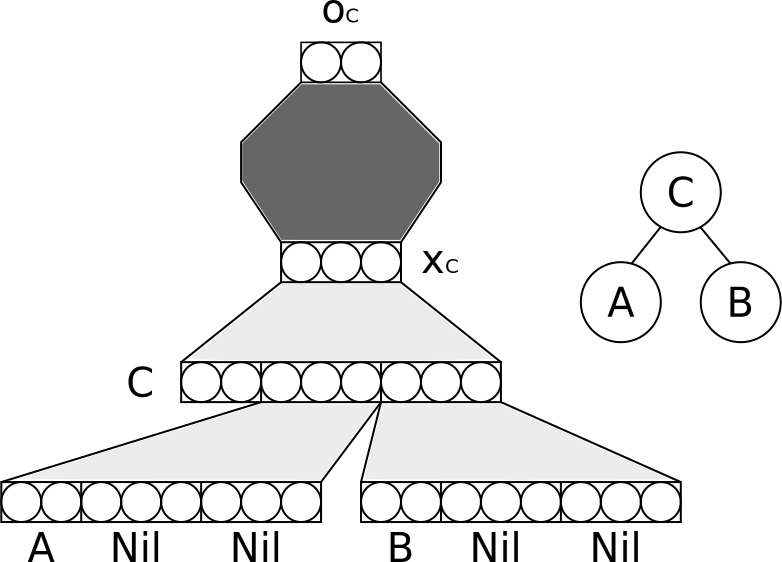
\includegraphics[scale=0.4]{img/virtual_unfolding}
	\caption{Virtual unfolding, reflecting the sample graph structure}
	\label{fig:virtual_unfolding}
\end{center}
\end{figure}

To explain the idea of BPTS it is necessary to briefly summarize the idea of BPTT (a detailed explanation can be found in RNN-concerned publications, e.g.~\cite{williams1995gradient}). Let's consider a fully-connected recurrent neural network, designed for classifying sequences of samples of size $m$. The network consists of a single layer of $n$ units with $n \times n$ recurrent connections, producing an output $\bm{y}(t)$ at time $t$. Let $\bm{x}^{s}(t)$ denote the $m$-tuple of input signals corresponding to the sample fed at time $t$. Further, let $\bm{x}(t)$ be the merged input fed to the network at time $t$, obtained by concatenating the vectors $\bm{x}^{s}(t)$ and $\bm{y}(t)$. To distinguish between the elements of vector $\bm{x}(t)$ corresponding to $\bm{x}^{s}(t)$ and to $\bm{y}(t)$, let's introduce two subsets of indices: $I$ and $U$ (Eq.~\ref{eq:bptt_indices}).

\begin{equation}
x_j(t) = \left\{
\begin{array}{l l}
	x^{s}_{j}(t)	& \quad \text{if $j \in I$} \\
	y_j(t)	& \quad \text{if $j \in U$}\\
\end{array} \right.
\label{eq:bptt_indices}
\end{equation}

\noindent Let $w_{kj}$ denote the network weight on connection to the $k$th neuron from input $x_j$, $net_k(t)$ denote the weighted sum of neuron inputs fed to the activation function of the $k$th neuron, $f_k$~(Eq.~\ref{eq:bptt_netk}) and $J(t)$ denote the overall mean square error of the network at time $t$.
\begin{equation}
net_k = \sum_{j \in (I \cup U)} w_{kj} x_j
\label{eq:bptt_netk}
\end{equation}

\begin{equation}
y_k = f_k(net_k)
\label{eq:bptt_f}
\end{equation}

\begin{equation}
J(t) = -\frac{1}{2} \sum_{k \in U} [e_k(t)]^2
\label{eq:bptt_j}
\end{equation}

\begin{equation}
e_k(t) = d_k(t) - y_k(t)
\label{eq:bptt_e}
\end{equation}

\noindent Let's consider a recurrent network which was operating from a starting time $t_0$ up to time $t$. We may represent the computation process performed by the network by \emph{unrolling} the network in time, that is building a feed-forward neural network made of identical instances of the considered recurrent neural network, one instance per time step $\tau$, $\tau \in (t_0, t]$. To compute the gradient of $J(t)$ at time $t$ it is necessary to compute values $\epsilon_k(\tau)$ and $\delta_k(\tau)$ for $k \in U$ and $\tau \in (t_0, t]$ by means of equations~\ref{eq:bptt_epsilon},~\ref{eq:bptt_delta} and~\ref{eq:bptt_summaric}.

\begin{equation}
\epsilon_k(t) = e_k(t)
\label{eq:bptt_epsilon}
\end{equation}

\begin{equation}
\delta_k(\tau) = f'_k(net_k(\tau))\epsilon_k(\tau)
\label{eq:bptt_delta}
\end{equation}

\begin{equation}
\epsilon_k(\tau - 1) = \sum_{j \in U} w_{jk} \delta_j(\tau)
\label{eq:bptt_summaric}
\end{equation}

\noindent Then, the gradient of $J(t)$ is calculated with respect to each weight $w_{ij}$ by the means of equation~\ref{eq:bptt_dj}.

\begin{equation}
\frac{\partial J(t)}{\partial w_{ij}} = \sum_{\tau = t_0 + 1}^{t} \delta_i(\tau) x_j(\tau - 1)
\label{eq:bptt_dj}
\end{equation}

\noindent At time $t$ an external error $\bm{e}(t)$ is \emph{injected} to the network, usually being the difference between the trained network output at time $t$: $\bm{y}(t)$ and the expected output $\bm{d}(t)$~(Eq.~\ref{eq:bptt_e}). The subsequent steps compute the error $\bm{\epsilon}(\tau)$ by backpropagating the original error through the layers of the unrolled neural network.

The BPTS method implements the BPTT algorithm. Backpropagation starts at the last layer of the virtual unfolding network, where the classification/regression error is calculated (the last layer of the transformation network applied to the root node). The error is injected to this layer and backpropagated using the BPTT algorithm down to the first layer of the folding network applied to the root node. The error is then backpropagated to the last layers of the folding network applied to the roots children, as if there was a physical connection. Such backpropagation continues down to the first layers of folding network applied to the terminal nodes.

The folding architecture model introduced new important ideas in the domain of connectionist graph processing models. First of all, the representation building model is simpler than the LRAAM model and the folding architecture converges much faster than LRAAM for the same datasets~\cite{goller1996learning}. Secondly, three important concepts were adapted from the domain of recurrent neural networks: the error injection, BPTS and the unfolding of the network as a generalisation of unrolling a recursive neural network.

\section{Generalised recursive neuron}
The \emph{generalised recursive neuron}, introduced in 1997~\cite{sperduti1997supervised} is a generalisation of the recurrent neuron, which in turn is used in recurrent neural networks (RNNs). It was created to provide an elementary component for the graph processing models which would be by definition better suited to solve graph processing tasks than the standard neuron. It is beyond the scope of this thesis to describe in detail the idea itself and its applications. Nevertheless this summary of the connectionist models would be incomplete without mentioning the generalised recursive neuron, as it was used in some of the following models instead of the common neural network neuron, yielding promising results~\cite{frasconi1998general}.

\noindent A generalised recursive neuron has two kinds of inputs:
\begin{itemize}
\item plain neuron inputs, which are fed with elements of the currently processed node label
\item recursive inputs, which are fed with the memorized output of the neuron for all children nodes of the currently processed node
\end{itemize}

\noindent In such a way, the neuron output changes after each training algorithm iteration, according to its output for all the children nodes.

\section{Recursive neural networks}
The folding architecture model had a large impact on a theory introduced in 1998, the \emph{structural transduction} formalism~\cite{frasconi1998general}. It is beyond the scope of this thesis to describe the formalism itself, let's mention however its aspects that highly affected the subsequent connectionist models described. The \emph{structural transduction}, in general, is a relation which maps a labelled DPAG (only node labels, no edge labels) into another DPAG. The type of transductions that the authors focus on are \emph{IO-isomorph} transductions, that is transductions that don't change the graph topology, only the node labels. (According to the authors managing transductions which are not \emph{IO-isomorph} is highly nontrivial and is an open research problem.) Let's describe an \emph{IO-isomorph} transduction. Let $G_s$ be the original DPAG with labelled nodes. Let $G_y$ be a graph with same topology that $G_s$ but with node labels replaced by expected node outputs for each node (it's a node classification/regression problem). A transduction $G_s \Rightarrow G_y$ can be described in terms of two functions, $f$ and $g$, where $f$ is the \emph{state transition function}, which builds the representation (the \emph{state}) $\bm{x}$ of the graph $G_s$ for the model and $g$ is the \emph{output function}, which produces the expected output graph $G_y$ according to the representation $\bm{x}$ and the original graph $G_s$. More precisely, for each node $i$ belonging to the original graph $G_s$ its state $\bm{x}_i \in \bm{x}$ and output ${\bm{y}}_i \in G_y$ are defined by Eq.~\ref{eq:recursive_state} and~\ref{eq:recursive_output}, where $\bm{l}_i$ is the $i$th node label and $\bm{x}_{ch[i]}$ is a vector obtained by stacking representations of all children of $i$th node one after another. In the original equations the $i$th node itself was also an argument of both functions, however, it was unnecessary from the point of view of recursive neural networks and therefore was omitted. 

\begin{equation}
\bm{x}_i = f(\bm{l}_i, \bm{x}_{ch[i]})
\label{eq:recursive_state}
\end{equation}

\begin{equation}
	\bm{y}_i = g(\bm{l}_i, \bm{x}_i)
\label{eq:recursive_output}
\end{equation}

The transduction can be implemented e.g. by a hidden recursive model (HRM) or by a \emph{recursive neural network} (a generalisation of a recurrent neural network, which is able to process not only sequences, but also DPAGs). In the case of a recursive neural network the functions $f$ and $g$ are implemented by two feed-forward neural networks. Identical instances of the $f$ network are connected according to the $G_s$ graph structure, creating the \emph{encoding network}. (The encoding network is the recursive neural network \emph{unfolded through the structure} of the given DPAG.) Calculation of the state $\bm{x}$ is performed by applying the $f$ network to the terminal nodes of $G_s$ and then proceeding up to the root, according to the encoding network topology. When the state calculation is finished, the $g$ network is applied to every node state $\bm{x}_i$, producing the requested output $\bm{y}_i$. A sample graph and the corresponding encoding network are presented in~Fig.~\ref{fig:recursive}.

\begin{figure}
\begin{center}
	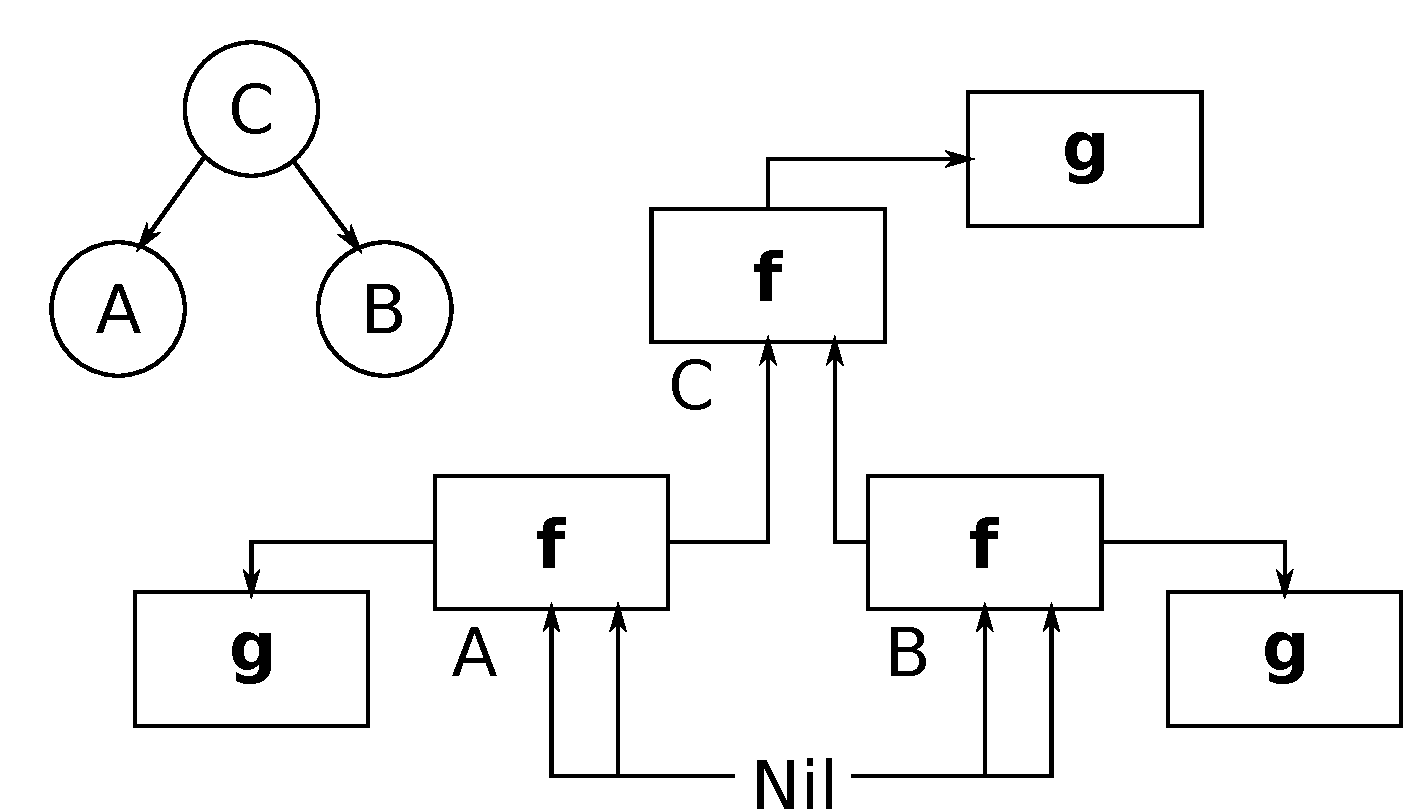
\includegraphics[scale=0.4]{img/encodinginc_recursive}
	\caption{A sample acyclic graph and the corresponding encoding network}
	\label{fig:recursive}
\end{center}
\end{figure}

As various kinds of neural network can be used as the $f$ function (first, second-order recurrent networks etc.), the recursive neural network model can become really complex and computationally powerful. However, for the scope of this work, it is sufficient to mention that the concepts of \emph{state transition function}, \emph{output function} and \emph{encoding network unfolded through structure} (originating from the \emph{folding architecture}) were later reused in the Graph Neural Network model. Another important feature of this model is a successful adaptation of ideas originating from recurrent neural network domain, just like in case of the \emph{folding architecture}. Authors of both models suggested that adaptation of other RNN ideas may also be possible, which could lead to novel graph processing solutions~\cite{kuchler1996inductive}~\cite{frasconi1998general}.


\chapter{Graph neural network implementation}

The Graph Neural Network model~\cite{scarselli2009graph} (GNN) is a quite recent (2009) connectionist model, based on recursive neural networks and capable of classifying almost all types of graphs. The main difference between the GNN model and previous connectionist models is the possibility of processing directly nonpositional and cyclic graphs, containing both node labels and edge labels. Although some similar solutions were introduced in an earlier model, the \emph{RNN-LE}~\cite{bianchini2005recursive} in 2005, it was the GNN model that combined several techniques with a novel learning schema to provide a direct and flexible method for graph processing.

\section{Data}
The GNN model is built once for a training set of graphs. In fact, a whole set of graphs can be merged into one large disconnected graph, which can then be fed to the model. For a given dataset each node $n$ is described by a node label $\bm{l}_n$ of fixed size $|\bm{l}_n| \geq 1$. Each directed edge $u \Rightarrow n$ (from node $u$ to node $n$) is described by an edge label $\bm{l}_{(n, u)}$ of fixed size $|\bm{l}_{(n, u)}| \geq 0$. To deal with both directed and undirected edges, the authors propose to include a value $d_l$ in each edge label, denoting the direction of an edge. However, for a maximally general model, in this implementation all the edges were considered as directed. Undirected edges were encoded prior to processing as pairs of directed edges with same labels.

A GNN model can deal with both \emph{graph-focused} and \emph{node-focused} tasks. In graph-focused tasks, for each graph an output $\bm{o}_n$ of fixed size $|\bm{o}_n| \geq 1$ is sought, which can denote e.g. the class of the graph. In the domain of chemistry, where each graph describes a chemical compound, this could describe e.g. the reactivity of a compound. In node-focused tasks, such output $\bm{o}_n$ is sought for every node in every graph. An example of such task can be the face localisation problem, where for each region of an image the classifier should determine, if it is a part of the face or not. In the rest of this thesis, the \emph{node-focused} task is described, unless stated otherwise.

For this implementation each graph was represented by three .csv files. Each $i$th row of the \emph{nodes file} contained the $i$th node label (comma-separated). Each row of the \emph{edges file} contained information about a directed edge $u \Rightarrow n$: the $u$ node index (row number in nodes file), the $n$ node index and the edge label (comma-separated). Each $i$th row of the \emph{outputs file} contained the $i$th node output (comma-separated). An example is provided in Appendix~\ref{chapter:using}.

\section{Computation units}
The GNN model consists of two computation units, $f_{\bm{w}}$ and $g_{\bm{w}}$, where the $_{\bm{w}}$ subscript denotes the fact that both units are functions parametrized by a vector of parameters $\bm{w}$, which is separate for the $f$ and for the $g$ function. The $f_{\bm{w}}$ unit is used for building representation (the \emph{state}) $\bm{x}_n$ of a single node $n$. The $g_{\bm{w}}$ unit is used for producing output $\bm{o}_n$ for a node $n$, basing on its representation $\bm{x}_n$. For a graph-focused task, the representation of the root node is fed to the $g_{\bm{w}}$ function to produce an output $\bm{o}_g$ for the whole graph. It is important to remind, that for a given classifier there is only one $f_{\bm{w}}$ unit and one $g_{\bm{w}}$ unit (like in the recursive neural network model). All instances of the $f_{\bm{w}}$ unit share their weights and all instances of the $g_{\bm{w}}$ unit share their weights.

Let's denote by $ne[n]$ the neighbors of node $n$, that is such nodes $u$ that are connected to node $n$ by a directed edge $u \Rightarrow n$. Let's further denote by $co[n]$ the set of directed edges pointing from $ne[n]$ towards node $n$ (edges $u \Rightarrow n$). The general forms of $f_{\bm{w}}$ and $g_{\bm{w}}$ functions are defined by equations Eq.~\ref{eq:gnn_f} and Eq.~\ref{eq:gnn_g}, where $\bm{l}_n$ denotes the $n$th node label, $\bm{l}_{co[n]}$ denotes the set of edge labels from $co[n]$, $\bm{x}_{ne[n]}$ denotes \emph{states} of nodes from $ne[n]$, and $\bm{l}_{ne[n]}$ denotes their labels.

\begin{equation}
\bm{x}_n = f_{\bm{w}}(\bm{l}_n, \; \bm{l}_{co[n]}, \; \bm{x}_{ne[n]}, \; \bm{l}_{ne[n]})
\label{eq:gnn_f}
\end{equation}

\begin{equation}
\bm{o}_n = g_{\bm{w}}(\bm{x}_n, \; \bm{l}_n)
\label{eq:gnn_g}
\end{equation}

\noindent For this implementation, minimal forms of these definitions were chosen:

\begin{equation}
\bm{x}_n = f_{\bm{w}}(\bm{l}_n, \; \bm{l}_{co[n]}, \; \bm{x}_{ne[n]})
\label{eq:gnn_fmin}
\end{equation}

\begin{equation}
\bm{o}_n = g_{\bm{w}}(\bm{x}_n)
\label{eq:gnn_gmin}
\end{equation}

These forms were chosen to prove that the model is capable of building a sufficient representation of each node. That is, the model should be able to encode all the necessary information from a node label $\bm{l}_n$ into the state $\bm{x}_n$. This approach proved later to be successful.

From two forms of the $f_{\bm{w}}$ function mentioned in the original article~\cite{scarselli2009graph}, the \emph{nonpositional form} was chosen. The reason behind this choice was to provide the model with the most general function possible, which could deal with both positional and nonpositional graphs. The nonpositional form was also the one yielding better results in the experiments conducted by the authors~\cite{scarselli2009graph}. The final definitions of the  $f_{\bm{w}}$ and $g_{\bm{w}}$ functions are shown below. All instances of the $h_{\bm{w}}$ unit share their weights.

\begin{equation}
\bm{x}_n = \sum_{u \in ne[n]}h_{\bm{w}}(\bm{l}_n, \; \bm{l}_{(n,u)}, \; \bm{x}_{u})
\label{eq:gnn_ffinal}
\end{equation}

\begin{equation}
\bm{o}_n = g_{\bm{w}}(\bm{x}_n)
\label{eq:gnn_gfinal}
\end{equation}

The units $h_{\bm{w}}$ and $g_{\bm{w}}$ were implemented as fully-connected three layer feed-forward neural networks (input lines performing no computation, a single hidden layer and an output layer). For both units the hidden layer consisted of $tanh$ neurons. For the $h_{\bm{w}}$ unit the output layer consisted of $tanh$ neurons. That's because the output of the $h_{\bm{w}}$ unit contributes to the state value and therefore should consist of bounded values only. For the $g_{\bm{w}}$ unit the output layer could consist either of $tanh$ or linear neurons, depending on the values of $\bm{o}_n$ that were to be learned.

At this point it's worth mentioning that the final value of $\bm{x}_n$ is calculated as a simple sum of $h_{\bm{w}}$ outputs. This corresponds to a situation where all the $h_{\bm{w}}$ output values are passed to a neural network in which the set of weights corresponding to a single $h_{\bm{w}}$ input are shared amongst all the $h_{\bm{w}}$ inputs. If we consider that a three layer FNN used as $h_{\bm{w}}$ unit is already an universal approximator, the use of such an additional neural network which just sums all $h_{\bm{w}}$ values using the same shared set of weights is unnecessary. A simple sum should be sufficient and experimental results showed that this assumption stands.

The $f_{\bm{w}}$ and $g_{\bm{w}}$ units are presented in Fig.~\ref{fig:gnn_f} and Fig.~\ref{fig:gnn_g}, where the comma-separated list of inputs stands for a vector obtained by stacking all the listed values one after another.

\begin{figure}[h!]
\begin{center}
	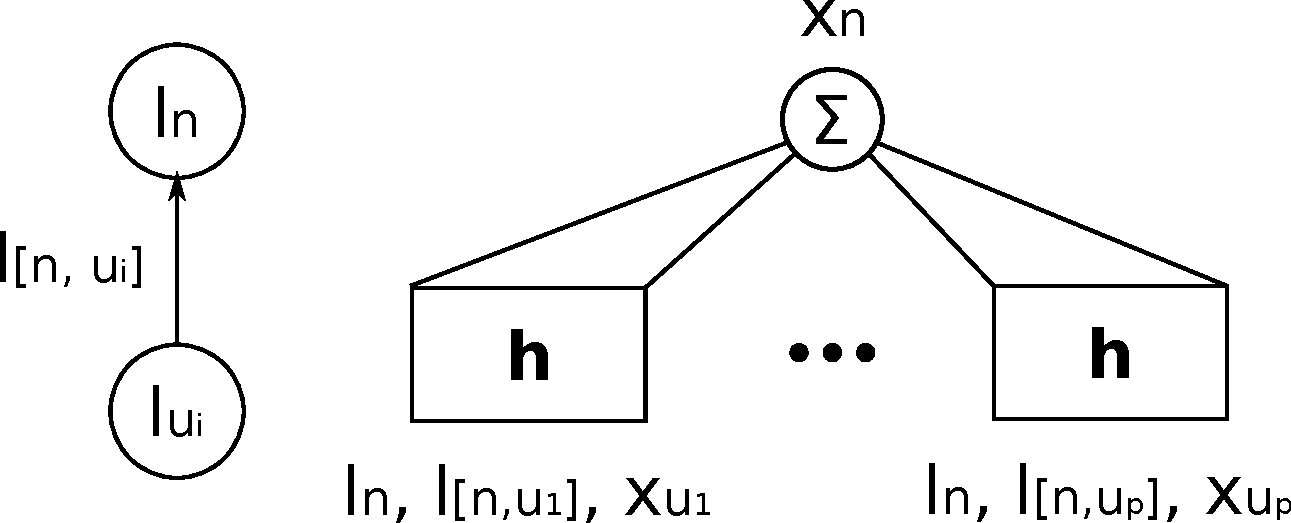
\includegraphics[scale=0.5]{img/f_ext}
	\caption{The $f_{\bm{w}}$ unit for a single node and one of the corresponding edges}
	\label{fig:gnn_f}
\end{center}
\end{figure}

\begin{figure}[h!]
\begin{center}
	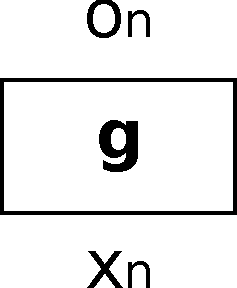
\includegraphics[scale=0.5]{img/g}
	\caption{The $g_{\bm{w}}$ unit for a single node}
	\label{fig:gnn_g}
\end{center}
\end{figure}

\newpage
The weights of both the $h_{\bm{w}}$ and $g_{\bm{w}}$ units were initialised according to the standard neural network practice, to avoid saturation of any $tanh$ activation function: $net_j = \sum_i w_{ji} y_i \in (-1, 1)$, where $net_j$ is the weighted input to $j$th neuron, $y_i$ is the $i$th input value and $w_{ji}$ is the weight corresponding to the $i$th input. The initial input weights of the $g_{\bm{w}}$ unit were divided by an additional factor, i.e. the maximum node indegree of the processed graphs, to take into consideration the fact, that the input of $g_{\bm{w}}$ unit consists of a sum of $h_{\bm{w}}$ outputs. All the input data (node and edge labels) was normalised appropriately before feeding to the model.


\section{Encoding network}
Graph processing by a GNN model consists of two steps: building representation $\bm{x}_n$ for each node and producing an output $\bm{o}_n$. As the representation of a single node depends on other nodes representations, an encoding network for every graph is built, reflecting the structure of the graph. The encoding network consists of instances of the $f_{\bm{w}}$ unit connected according to the graph structure with a $g_{\bm{w}}$ unit attached to every $f_{\bm{w}}$ unit. A sample graph and its encoding network are presented in Fig.~\ref{fig:gnn_encoding}.
It can be seen that, as a cyclic dependence exists in the sample graph, the calculation of the node \emph{states} should be iterative, until at some point convergence is reached.

\begin{figure}[h!]
\begin{center}
	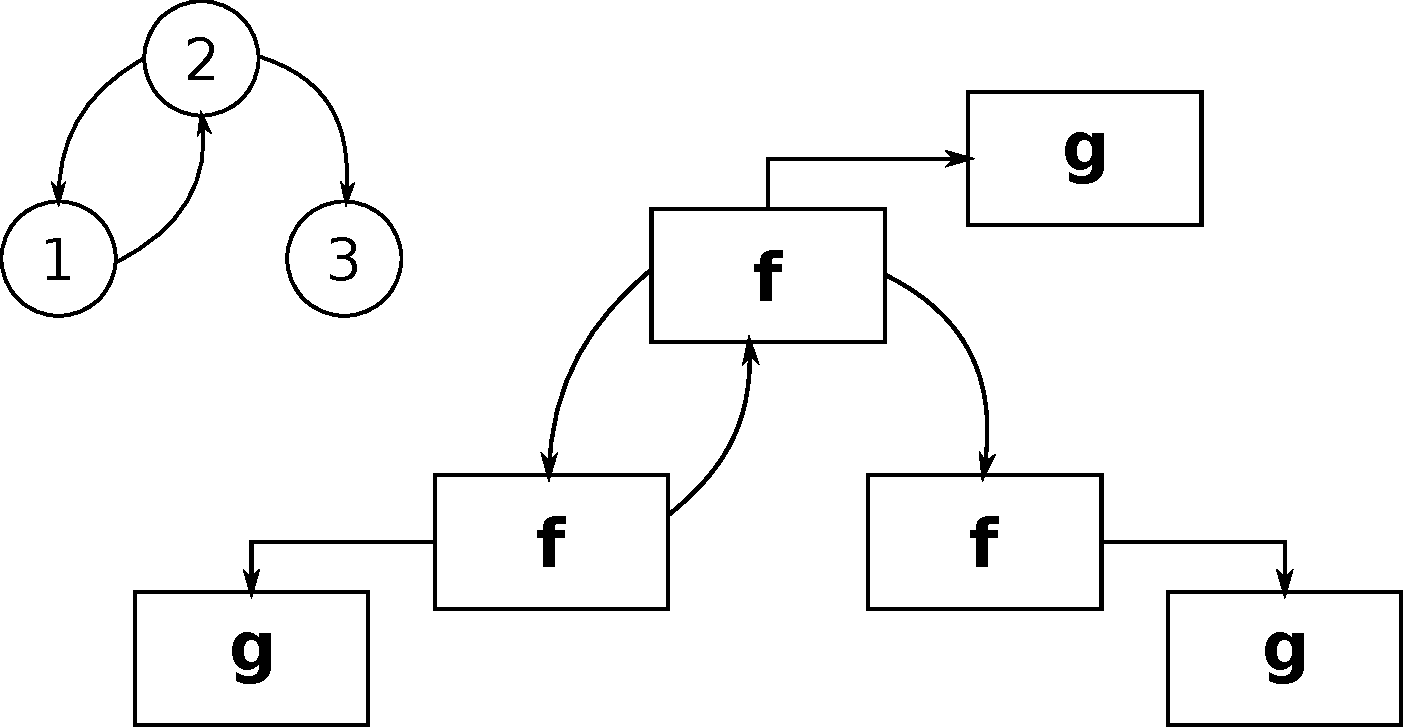
\includegraphics[scale=0.4]{img/encodinginc}
	\caption{A sample graph and the corresponding encoding network}
	\label{fig:gnn_encoding}
\end{center}
\end{figure}


\section{General training algorithm}
Let's denote by $\bm{x}$ the \emph{global state} of the graph, that is the set of all $\bm{x}_n$ for every node $n$ in the graph. Let's denote by $\bm{l}$ and $\bm{o}$ the sets of all labels and all outputs, respectively. Let's further denote by $F_{\bm{w}}$ and $G_{\bm{w}}$ (\emph{global transition function} and \emph{global output function}) the stacked versions of $f_{\bm{w}}$ and $g_{\bm{w}}$ functions, respectively. Now, equations~\ref{eq:gnn_fmin} and~\ref{eq:gnn_gmin} can be rewritten as Eq.~\ref{eq:gnn_fglobal} and Eq.~\ref{eq:gnn_gglobal}.

\newpage
\begin{equation}
\bm{x} = F_{\bm{w}}(\bm{l}, \; \bm{x})
\label{eq:gnn_fglobal}
\end{equation}

\begin{equation}
\bm{o} = G_{\bm{w}}(\bm{x})
\label{eq:gnn_gglobal}
\end{equation}

\noindent The GNN training algorithm can be described as follows:
\begin{enumerate}
	\item initialize $h_{\bm{w}}$ and $g_{\bm{w}}$ weights
	\item until stop criterion is satisfied:
	\begin{enumerate}
		\item initialize $\bm{x}$ randomly
		\item FORWARD: calculate $\bm{x} = F_{\bm{w}}(\bm{l}, \; \bm{x})$ until convergence
		\item BACKWARD: calculate $\bm{o} = G_{\bm{w}}(\bm{x})$ and backpropagate the error
		\item update $h_{\bm{w}}$ and $g_{\bm{w}}$ weights
	\end{enumerate}
\end{enumerate}
\noindent The stop criterion used in this implementation was a maximum number of iterations.


\section{Unfolded network and backpropagation}
To solve the problem of cyclic dependencies, the GNN models adapts a novel learning algorithm for the encoding network. The encoding network is virtually \emph{unfolded} through time until at time $t_m$ the state $\bm{x}$ converges to a \emph{fixed point} $\hat{\bm{x}}$ of the function  $F_{\bm{w}}$. Then the output $\bm{o}$ is calculated. Such unfolded network for the sample graph is presented in Fig.~\ref{fig:gnn_forward}. Each time step consists of evaluating the $f_{\bm{w}}$ function at every node. What is important, the connections between nodes are taken into consideration only between time steps. In such a way, the problem of cycles ceases to exist and the processed graph can be even fully connected.

\begin{figure}[h!]
\begin{center}
	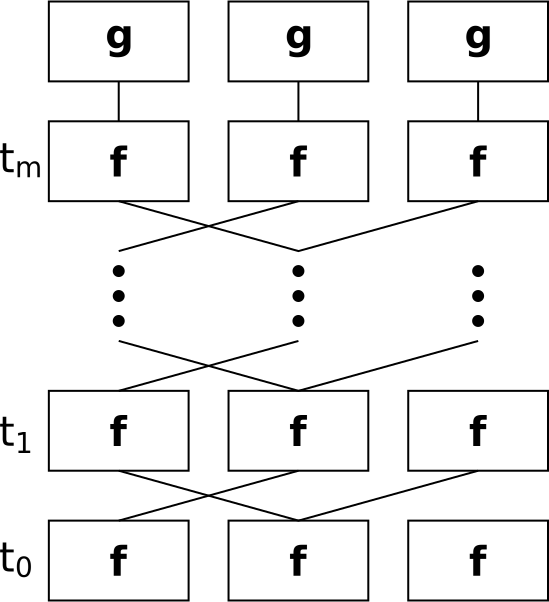
\includegraphics[scale=0.4]{img/forward}
	\caption{Unfolded encoding network for the sample graph}
	\label{fig:gnn_forward}
\end{center}
\end{figure}

After the output $\bm{o}$ is calculated, the error $e_n = (d_n - o_n)^2$ is injected to the corresponding $g_{\bm{w}}$ unit for every node $n$, where $d_n$ denotes the expected node output. The error is backpropagated through the $g_{\bm{w}}$ layer, yielding the value $\frac{\partial e_{\bm{w}}}{\partial \bm{o}}\cdot \frac{\partial G_{\bm{w}}}{\partial x}(\hat{\bm{x}})$. That value is backpropagated through the unfolded network using the BPTT/BPTS algorithm. Additionally, at each time step the $\frac{\partial e_{\bm{w}}}{\partial \bm{o}}\cdot \frac{\partial G_{\bm{w}}}{\partial x}(\hat{\bm{x}})$ error is injected to the $f_{\bm{w}}$ layer, as presented in Fig.~\ref{fig:gnn_backward}. In such a way the error backpropagated through the $f_{\bm{w}}$ layer at time $t_i$ comes from two sources. First, it is the output error of the network $\frac{\partial e_{\bm{w}}}{\partial \bm{o}}\cdot \frac{\partial G_{\bm{w}}}{\partial x}(\hat{\bm{x}})$. Secondly, it is the error backpropagated from the subsequent time layers of the $f_{\bm{w}}$ unit from all nodes connected with the given node $u$ by an edge $u \Rightarrow n$.

\begin{figure}[h!]
\begin{center}
	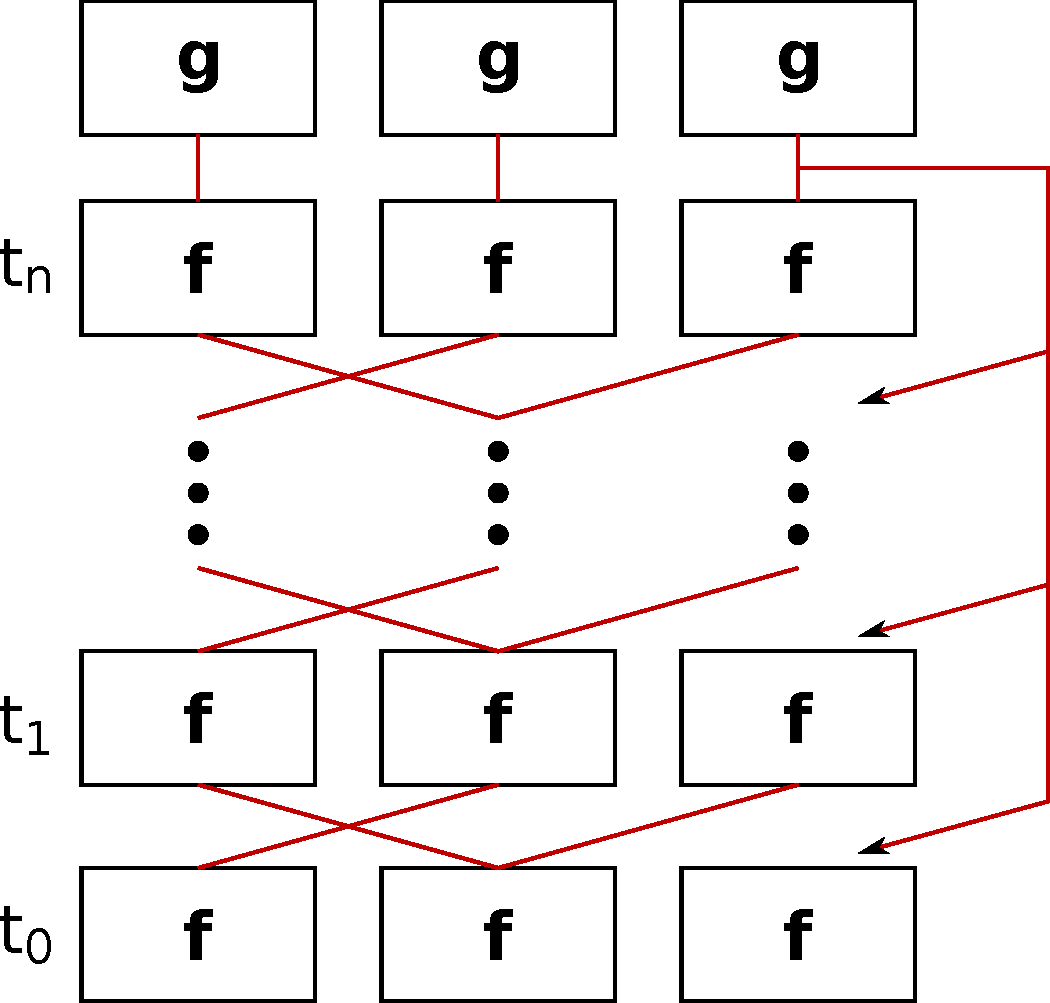
\includegraphics[scale=0.4]{img/backward}
	\caption{Error backpropagation through the unfolded network}
	\label{fig:gnn_backward}
\end{center}
\end{figure}

By injecting the same error $\frac{\partial e_{\bm{w}}}{\partial \bm{o}}\cdot \frac{\partial G_{\bm{w}}}{\partial x}(\hat{\bm{x}})$ at each time step an important assumption is made, which leads to a simplification of the whole backpropagation process. If the state $\bm{x}$ converged to a \emph{fixed point} $\hat{\bm{x}}$ of function $F_{\bm{w}}$ at time $t_m$, then it can be safely assumed that using the value $\hat{\bm{x}}$ at every previous time step $t_i$ instead of $\bm{x}(t_i)$ would yield the same result at time $t_m$.

Storing the intermediate values of $\bm{x}(t_i)$ and backpropagating the error directly using the BPTT/BPTS algorithm would be memory consuming. However, due to the assumption that $\bm{x}(t_i) = \hat{\bm{x}}$, a different backpropagation algorithm can be used~\cite{scarselli2009graph}, originating from the domain of recurrent neural networks: the Almeida-Pineda algorithm~\cite{pineda1987generalization}~\cite{williams1995gradient}.

Basically, the modified Almeida-Pineda algorithm consists of initializing an \emph{error accumulator} $\bm{z}(0) = \frac{\partial e_{\bm{w}}}{\partial \bm{o}}\cdot \frac{\partial G_{\bm{w}}}{\partial x}(\hat{\bm{x}})$ and then accumulating the error by backpropagating $\bm{z}(j)$ through the $f_{\bm{w}}$ layer until its value converges to $\hat{\bm{z}}$. At each step $j$ the additional error $\frac{\partial e_{\bm{w}}}{\partial \bm{o}}\cdot \frac{\partial G_{\bm{w}}}{\partial x}(\hat{\bm{x}})$ is injected as was shown previously. If the state calculation converged, the error calculation is guaranteed to converge too. The number of iterations needed for the \emph{error accumulator} $\bm{z}$ to converge can be different than the number of time steps needed for the state $\bm{x}$ to converge. In the conducted experiments it was usually much smaller.


\section{Contraction map\label{sec:contraction}}
In the previous paragraphs, it was stated that a fixed point $\hat{\bm{x}}$ of function $F_{\bm{w}}$ is sought. However, how can it be assumed that such a fixed point exists for the function $F_{\bm{w}}$? How to assure that it will be reached by iterating $\bm{x} = F_{\bm{w}}(\bm{x})$ using a random initial $\bm{x}$?

Actually all of the above can be assured by making $F_{\bm{w}}$ a \emph{contraction map}. A \emph{contraction map} (a \emph{non-expansive} map) is a function $F_{\bm{w}}$ for which $d(F_{\bm{w}}(\bm{x}_1), \; F_{\bm{w}}(\bm{x}_2)) \leq d(\bm{x}_1, \; \bm{x}_2)$, where $d(\bm{x}, \; \bm{y})$ is a distance function. For this implementation a distance function $d(\bm{x}, \; \bm{y}) = max_i(|x_{i} - y_{i}|)$ was chosen, as it is independent of the \emph{state} size and therefore, of the number of nodes in a given graph. The \emph{Banach Fixed Point Theorem} states that a contraction map $F_{\bm{w}}(\bm{x})$ has the following properties:
\begin{itemize}
	\item it has a single fixed point $\hat{\bm{x}}$
	\item it converges to $\hat{\bm{x}}$ from every starting point $\bm{x}(t_0)$
	\item the convergence to  $\hat{\bm{x}}$ is exponentially fast~\cite{scarselli2009graph}.
\end{itemize}

\noindent How to assure that $F_{\bm{w}}$, a function composed of neural network instances, is actually a contraction map? The authors propose to impose a penalty function whenever the elements of the Jacobian $\frac{\partial F_{\bm{w}}}{\partial \bm{x}}$ suggest that $F_{\bm{w}}$ isn't a contraction map anymore.

Let $\bm{A} = \frac{\partial F_{\bm{w}}}{\partial \bm{x}}(\bm{x}, \; \bm{l})$ be a block matrix of size $N \times N$ with blocks of size $s \times s$, where $N$ is the number of nodes in the processed graph and $|\bm{x}_n| = s$ is the state size for a single node. A single block $\bm{A}_{n,u}$ measures the influence of the node $u$ on node $n$ if an edge from $u$ to $n$ exists or is zeroed otherwise. Let's denote by $I_u^j$ the influence of node $u$ on the $j$th element of state $\bm{x}_n$ (Eq.~\ref{eq:gnn_pw_inf}). The penalty $p_{\bm{w}}$ added to the network error $e_{\bm{w}}$ is defined by Eq.~\ref{eq:gnn_pw}.

\begin{equation}
p_{\bm{w}} = \sum_{u \in N} \sum_{j = 1}^{s} L(I_u^j, \; \mu)
\label{eq:gnn_pw}
\end{equation}

\begin{equation}
L(y, \; \mu) = \left\{
\begin{array}{l l}
	y - \mu		& \quad \text{if $y > \mu$} \\
	0			& \quad \text{otherwise}
\end{array} \right.
\label{eq:gnn_pw_L}
\end{equation}

\begin{equation}
I_u^j =  \sum_{(n, u)} \sum_{i = 1}^{s} |\bm{A}_{n, u}^{i, j}|
\label{eq:gnn_pw_inf}
\end{equation}

Basing on these equations, the value of $\frac{\partial p_{\bm{w}}}{\partial \bm{w}}$ is calculated and the final error derivative for the $h_{\bm{w}}$ network is calculated as $\frac{\partial e_{\bm{w}}}{\partial \bm{w}} + \frac{\partial p_{\bm{w}}}{\partial \bm{w}}$. It can be seen from Eq.~\ref{eq:gnn_pw_L} that the  term $\frac{\partial p_{\bm{w}}}{\partial \bm{w}}$ affects only weights that cause an excessive impact (larger than $\mu$) and the value of such penalty is proportional to the value of $I_u^j$. The eagerness to impose the penalty and the penalty value are inversely proportional to the value of the \emph{contraction constant} $\mu$. The impact of \emph{contraction constant} on the training process was described in section~\ref{sec:contraction_constant}.

\newpage
\section{RPROP algorithm}
The authors of the GNN algorithm suggest the RPROP algorithm~\cite{riedmiller1993direct} as the weights update algorithm, as an efficient gradient descent strategy. The basic idea of the RPROP algorithm is to use only the sign of the original weight updates $\frac{\partial e_{\bm{w}}}{\partial \bm{w}}$. The actual weight updates are calculated by the RPROP algorithm according to the past behaviour of $\frac{\partial e_{\bm{w}}}{\partial \bm{w}}$, which includes fast descent of monotonous gradient slopes, small steps in the proximity of a minimum and reverting updates that caused jumping over a local minimum. Actually, in the case of GNN, the RPROP algorithm should be used not only for its efficiency, but also as a way of dealing with the unpredictable behaviour of the $\frac{\partial p_{\bm{w}}}{\partial \bm{w}}$ term. As experiments showed, the value of $\frac{\partial p_{\bm{w}}}{\partial \bm{w}}$ can be larger than the original $\frac{\partial e_{\bm{w}}}{\partial \bm{w}}$ by several orders of magnitude, which could disturb severely the learning algorithm if the RPROP algorithm wasn't used. The RPROP algorithm was implemented using standard recommended values~\cite{riedmiller1993direct}, with the exception of $\Delta_{max}$ which was set to $1$ to avoid large weight changes.


\section{Maximum number of iterations}
As was shown in section~\ref{sec:contraction}, the number of \emph{Forward} or \emph{Backward} steps is finite if $F_{\bm{w}}$ is a contraction map. However, it can be seen, that the penalty imposed on the weights is in fact imposed post factum. Only after the norm of the Jacobian $\frac{\partial F_{\bm{w}}}{\partial \bm{x}}$ increases excessively, the penalty is imposed. In fact:
\begin{enumerate}
	\item it is not guaranteed that the Jacobian norm will be correct after the penalty is imposed
	\item one \emph{Forward} iteration takes place before the penalty is imposed
\end{enumerate}
Even if the penalty is efficient enough (it isn't necessarily so, as shown in the subsequent experiments), the problem of a single \emph{Forward} iteration that may not converge still remains. During experiments it was observed that while usually the number of \emph{Forward} iterations was between 5 and 50, depending on the dataset, from time to time it reached about 2000 iterations or even more (the calculations had to be aborted due to excessive time). To make the calculation time predictable it was necessary to introduce a modification to the original GNN algorithm - a maximum number of \emph{Forward} iterations. The value chosen for the subsequent experiments was 200, as it seemed to be a value large enough (in comparison to the usual number of steps) to assure that the state calculation will converge if $F_{\bm{w}}$ is still a contraction map. Furthermore, if the state calculation doesn't converge, it is not guaranteed that the error accumulation calculation will. Therefore, another similar restriction was introduced for the \emph{Backward} procedure and the maximum number of \emph{Backward} (error accumulation) iterations was set to 200. 

\newpage
\section{Detailed training algorithm}
\begin{lstlisting}[mathescape, style=outcode, language=pascal, caption=The learning algorithm]
MAIN:
	$\bm{w} = \text{initialize}$
	$\bm{x} = FORWARD(\bm{w})$
	for $numberOfIterations$:
		$[\frac{\partial eh_{\bm{w}}}{\partial \bm{w}}; \; \frac{\partial eg_{\bm{w}}}{\partial \bm{w}}] = BACKWARD(\bm{x}, \; \bm{w})$
		$\bm{w} = \text{rprop-update}(\bm{w}, \; \frac{\partial eh_{\bm{w}}}{\partial \bm{w}}, \; \frac{\partial eg_{\bm{w}}}{\partial \bm{w}})$
		$\bm{x} = FORWARD(\bm{w})$
	end
	return $\bm{w}$
end

FORWARD($\bm{w}$):
	$\bm{x}(0) = \text{random}$
	$t = 0$
	repeat:
		$\bm{x}(t+1) = F_{\bm{w}}(\bm{x}(t), \; \bm{l})$
		$t = t + 1$
	until $(max_i(|x_i(t + 1) - x_i(t)|) \leq minStateDiff)$ or $(t > maxForwardSteps)$
	return $\bm{x}(t)$
end

BACKWARD($\bm{x}$, $\bm{w}$):
	$\bm{o} = G_{\bm{w}}(\bm{x})$
	$\bm{A} = \frac{\partial F_{\bm{w}}}{\partial \bm{x}}(\bm{x}, \; \bm{l})$
	$\bm{b} = \frac{\partial e_{\bm{w}}}{\partial \bm{o}}\cdot \frac{\partial G_{\bm{w}}}{\partial x}(\bm{x})$
	$\bm{z}(0) = \bm{b}$
	$t = 0$
	repeat:
		$\bm{z}(t - 1) = \bm{z}(t) \cdot \bm{A} + \bm{b}$
		$t = t - 1$
	until $(max_i(|z_i(t - 1) - z_i(t)|) \leq minErrorAccDiff)$ or $(|t| > maxBackwardSteps)$
	$\frac{\partial eg_{\bm{w}}}{\partial \bm{w}} = b$
	$\frac{\partial eh_{\bm{w}}}{\partial \bm{w}} = \bm{z}(t) \cdot \frac{\partial F_{\bm{w}}}{\partial \bm{w}}(\bm{x}, \bm{l}) + \frac{\partial p_{\bm{w}}}{\partial \bm{w}}$
	return $[\frac{\partial eh_{\bm{w}}}{\partial \bm{w}}; \; \frac{\partial eg_{\bm{w}}}{\partial \bm{w}}]$
end
\end{lstlisting}

\section{Graph-focused tasks}
The GNN model can be used for graph-focused tasks by modifying the standard learning algorithm. In a graph-focused task an output $\bm{o}_g$ is sought for every graph, which is the output of a predefined root node. In such a task only the root output error can be measured, as for every other node the expected output is not defined. Thus, the only modification necessary to deal with such a task is to set the error of all non-root nodes to zero. Such a modification was implemented and proved to work well for a modified subgraph matching task (see chapter~\ref{ch:experiments}), where the modified task consisted of determining if a given graph contains the expected subgraph $S$ or not instead of selecting nodes belonging to $S$.


\chapter{Experiments~\label{ch:experiments}}
Experiments were conducted to check if the implemented GNN is able to cope with the tasks presented in the original article~\cite{scarselli2009graph}. For all the experiments the state size was set to 5, the number of hidden neurons in both the $h_{\bm{w}}$ and $g_{\bm{w}}$ networks was set to 5. After some successful trivial experiments, consisting of memorizing a single graph, the proper experiments were conducted. The task chosen for experiments was the \emph{subgraph matching} task. It was chosen, because:
\begin{enumerate}
	\item a similar experiment was conducted by Scarselli et al.~\cite{scarselli2009graph}
	\item the dataset is easy to generate, yet the problem is not trivial
	\item to yield good results, the structure of the graph have to be exploited.
\end{enumerate}

\section{Subgraph matching - data}
The datasets for the subgraph matching task were generated as follows. For a given number of graph nodes, graphs were generated by selecting node labels from $[0..10]$ and connecting each node pair in a graph with an edge probability $\delta$. Then, edges were inserted randomly until the graph became connected. Then, a smaller (connected) subgraph $S$ was inserted to every graph in the dataset. Then, a brute force algorithm was used to locate all copies of the subgraph $S$ in every graph in the dataset. Thus, every graph in the dataset contained at least on copy of the subgraph $S$. Afterwards, a small Gaussian noise with zero mean and standard deviation of $0.25$ was added to all node labels. All graph edges were undirected and thus were transformed to pairs of directed edges prior to processing. No edge labels were used.

Two datasets were generated. One with graph size (number of nodes) equal to 6, the subgraph size equal to 3 and $\delta = 0.8$ (100 graphs, called later the \emph{6-3 dataset}). The second dataset with graph size equal to 14, subgraph size equal to 7 and $\delta = 0.2$ (100 graphs, called later the \emph{14-7 dataset}). A larger $\delta$ was used for the first dataset, as graphs generated with $\delta = 0.2$ were mostly sequences. The first dataset was used to analyze the process of training, while the second one was used for comparison of GNN with a standard FNN classifier.

\begin{figure}[h!]
\begin{center}
	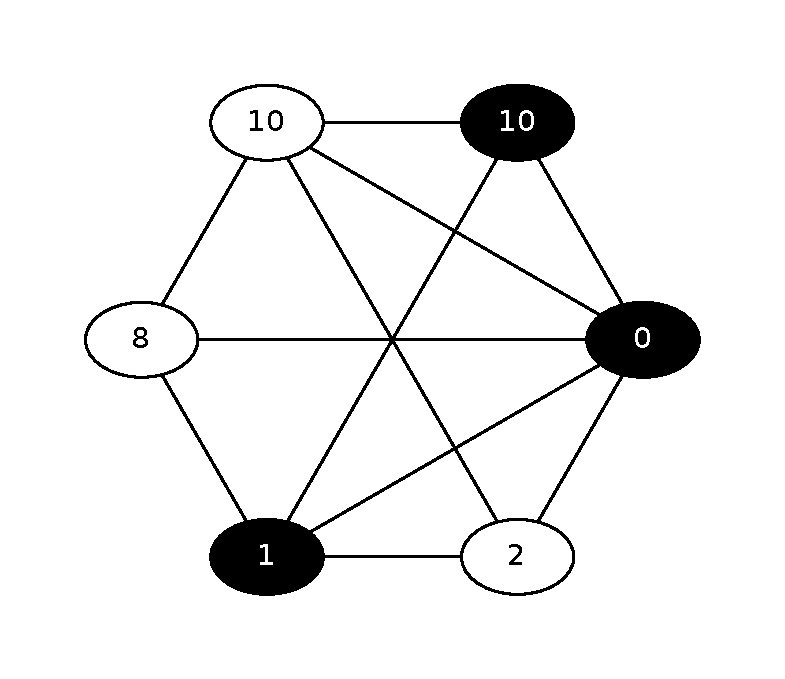
\includegraphics[scale=0.6]{img/g6s3_1.pdf}
	\caption{Sample graph from 6-3 dataset (subgraph in black), before adding noise}
	\label{fig:gnn_g6s3}
\end{center}
\end{figure}

\begin{figure}[h!]
\begin{center}
	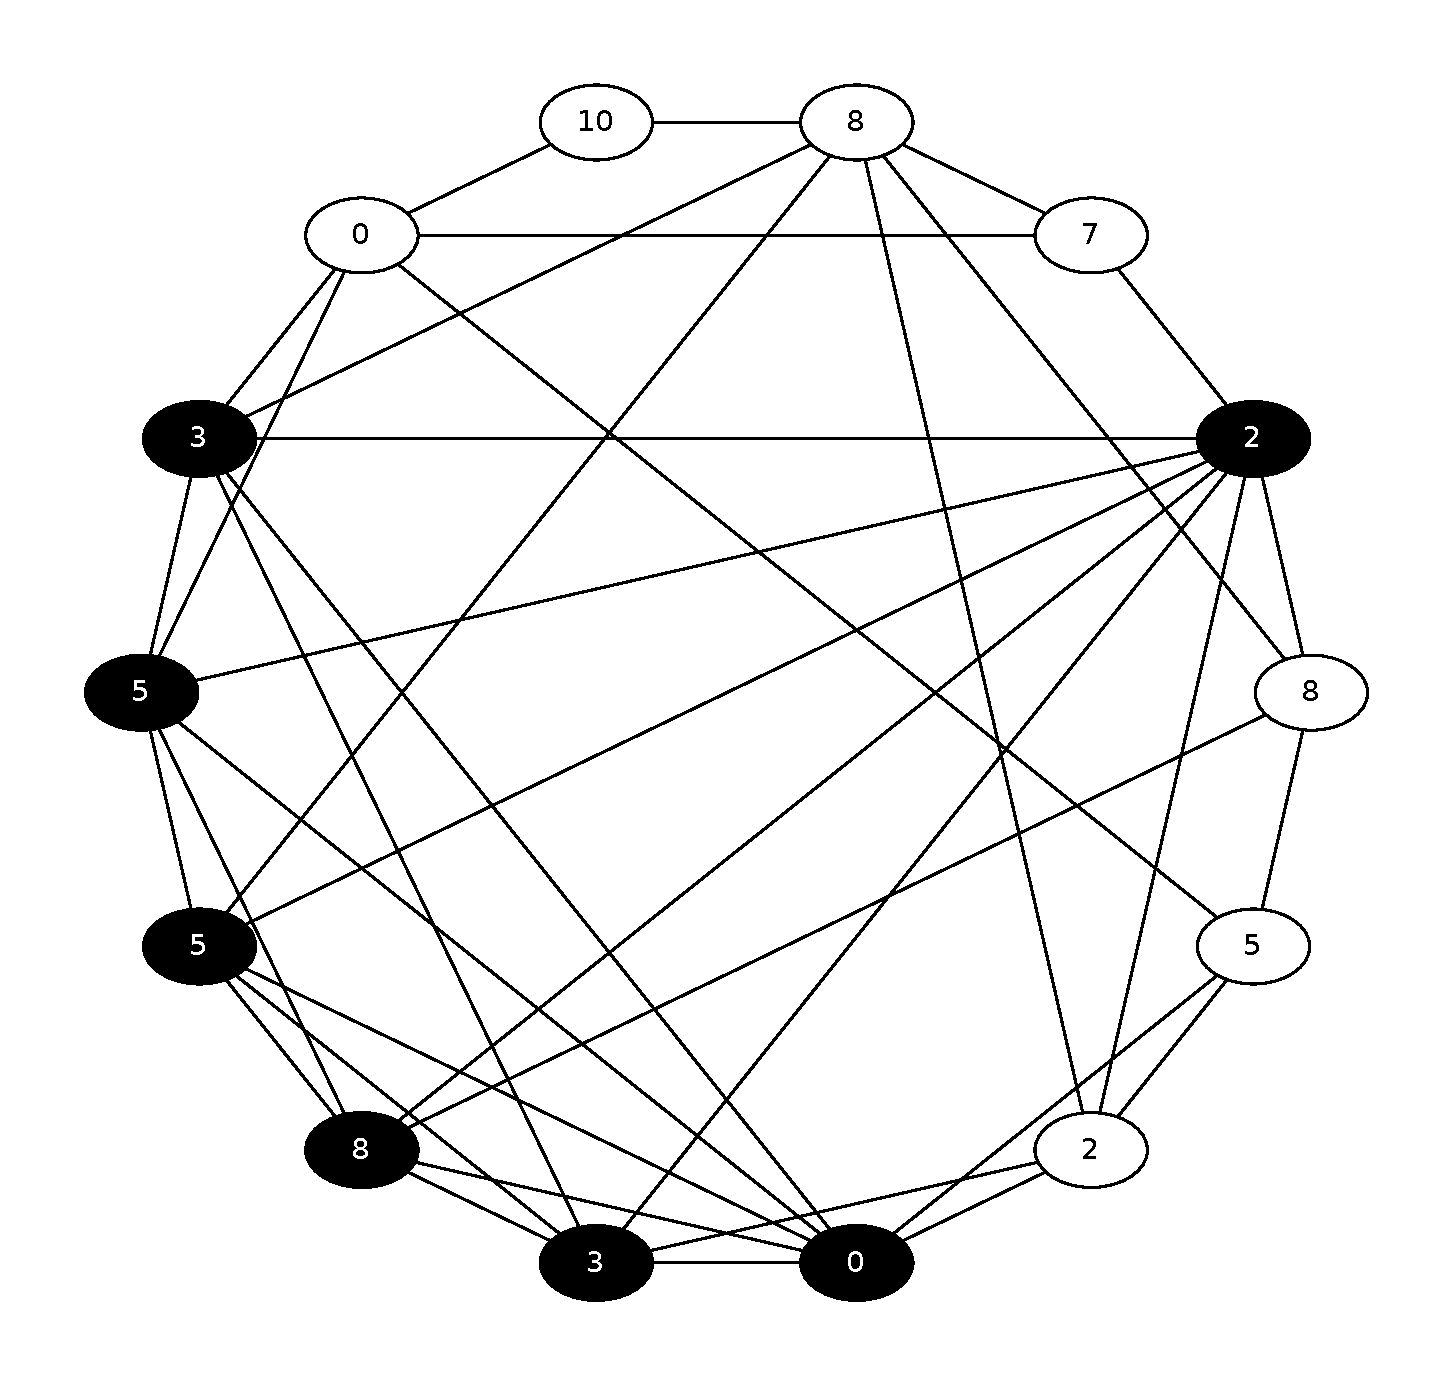
\includegraphics[scale=0.6]{img/g14s7_7.pdf}
	\caption{Sample graph from 14-7 dataset (subgraph in black), before adding noise}
	\label{fig:gnn_g6s3}
\end{center}
\end{figure}

\newpage
\section{Impact of initial weight values on learning}
To test the impact of initial weight values on the process of a GNN training, 9 different sets of weights were tested. For all tested networks, the contraction constant ($\mu$ from Eq.~\ref{eq:gnn_pw}) was set to $0.9$. The training was performed on 10 graphs belonging to the 6-3 dataset. Each GNN network was trained for 50 iterations. As the default error measure used in GNN training is the Mean Square Error, a similar performance measure - RMSE was used for evaluation. Results are presented in Fig.~\ref{fig:gnn_multiple}. Out of 9 networks, only 4 performed well: gnn2, gnn3, gnn5 and gnn7. The gnn5 network yielded the smallest RMSE at the end of training and also presents a remarkably monotonous RMSE slope compared to gnn7. All the other networks didn't improve significantly on the RMSE value, which may suggest that multiple initial sets of weights should be tried for a given dataset to build an efficient classifier.

\begin{figure}[h!]
\begin{center}
	\includegraphics[scale=0.09]{img/rmse_gnn1-9}
	\caption{RMSE for 9 different initial weight sets. $\mu = 0.9$}
	\label{fig:gnn_multiple}
\end{center}
\end{figure}

\newpage
\section{Impact of contraction constant on learning~\label{sec:contraction_constant}}
During the initial experiments, interesting results were obtained for different values of the contraction constant ($\mu$ from Eq.~\ref{eq:gnn_pw}). It seems that for a given learning task exists a minimum value of $\mu$ below which no learning occurs. Some experiments were conducted for the 6-3 dataset using the best networks from Fig.~\ref{fig:gnn_multiple}: the gnn5 and gnn7 network (initial weight values were used). The results for gnn7 are presented in Fig.~\ref{fig:gnn7} and the results for gnn5 are presented in Fig.~\ref{fig:gnn5}. For both networks three different values of $\mu$ were tested: 1.2, 0.9 and 0.6. In both cases it can be observed that no training occurs for $\mu = 0.6$. For these experiments 20 graphs from the 6-3 dataset were used.

\begin{figure}[h!]
\begin{center}
	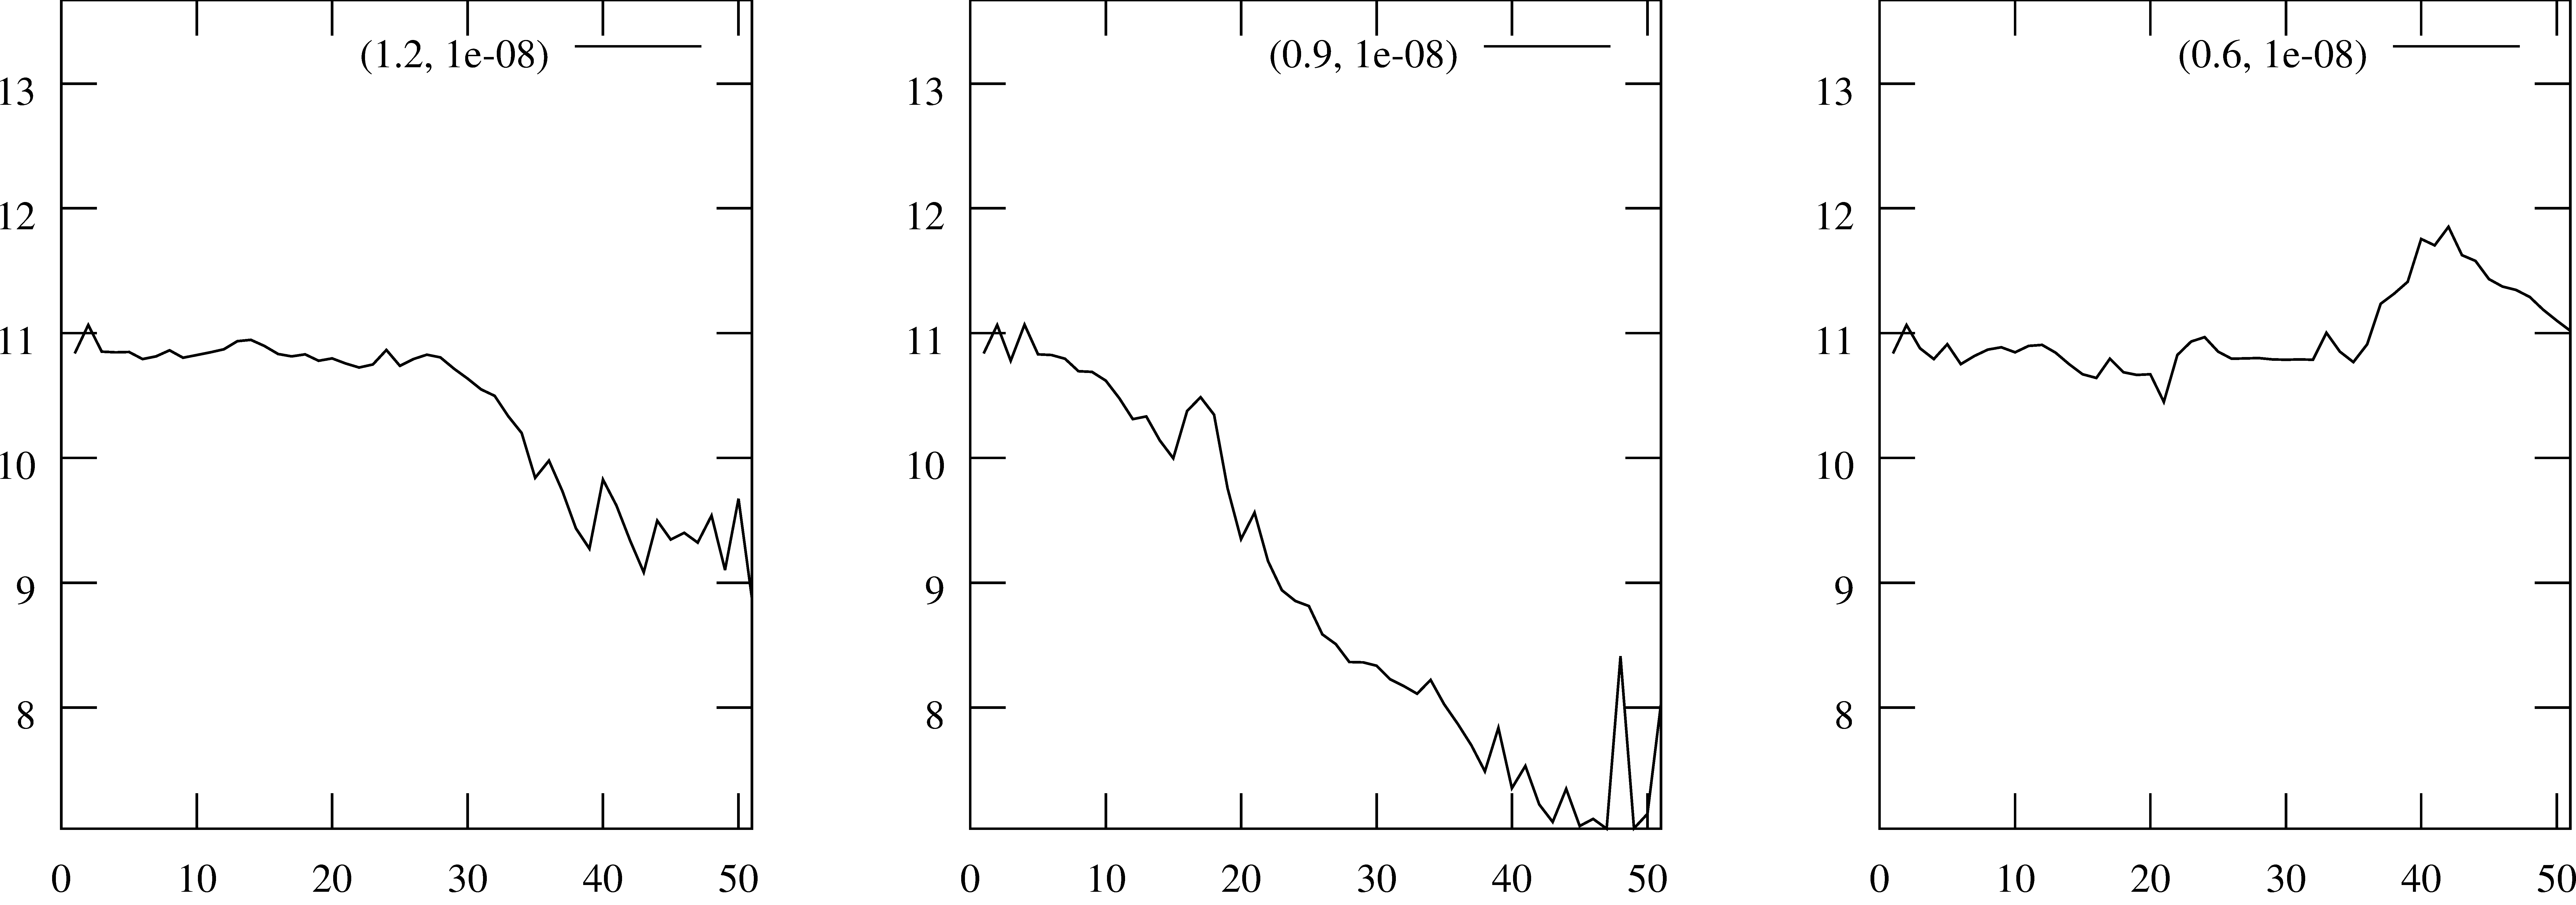
\includegraphics[scale=0.09]{img/rmse_clipped}
	\caption{RMSE for gnn7 with $\mu \in [1.2, 0.9, 0.6]$}
	\label{fig:gnn7}
\end{center}
\end{figure}

\begin{figure}[h!]
\begin{center}
	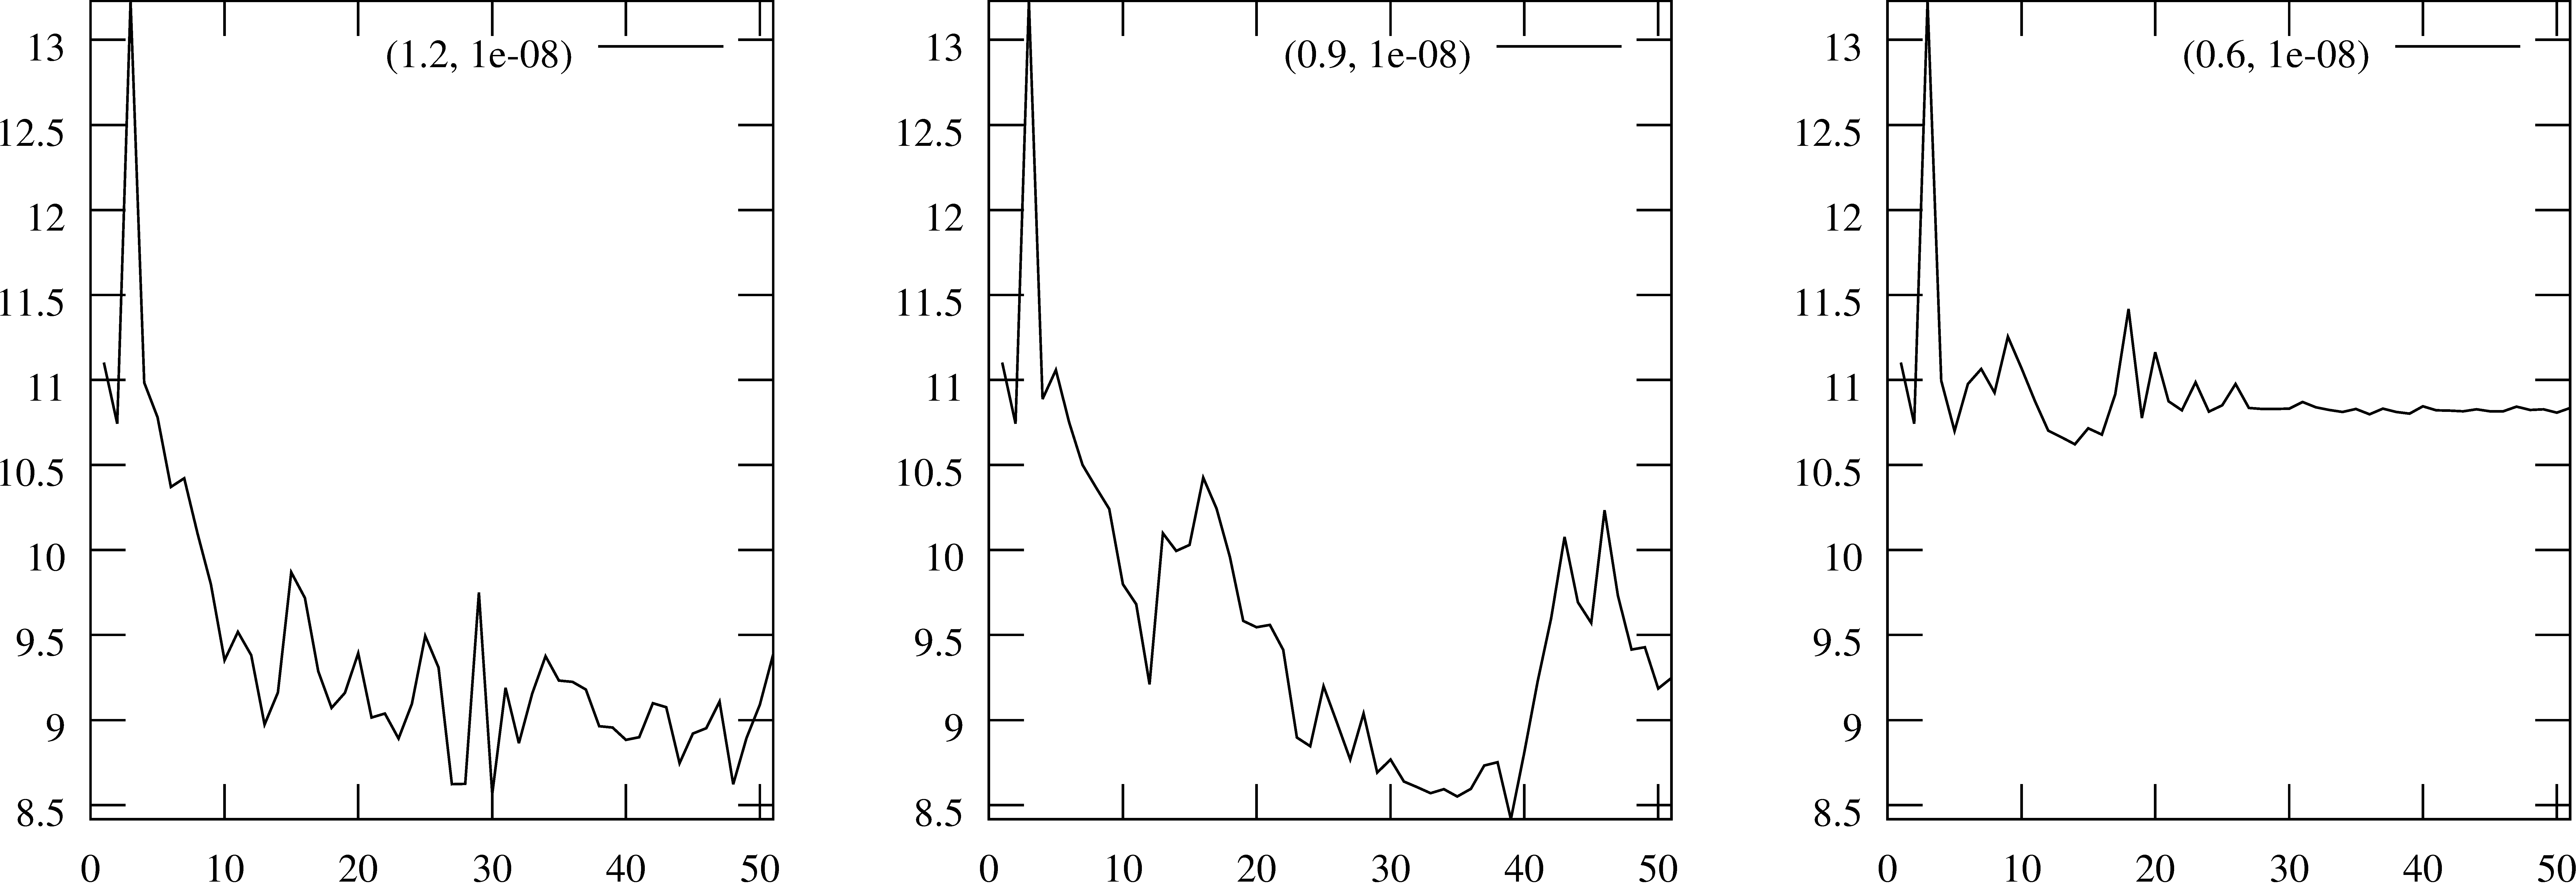
\includegraphics[scale=0.09]{img/rmse1a_clipped}
	\caption{RMSE for gnn5 with $\mu \in [1.2, 0.9, 0.6]$}
	\label{fig:gnn5}
\end{center}
\end{figure}

A closer look on the process of learning may shed some light on the reasons behind the lack of learning. In Fig.~\ref{fig:gnn5_09} the process of learning of gnn5 with $\mu = 0.9$ is presented. In Fig.~\ref{fig:gnn5_06} the same network gnn5 was trained with $\mu = 0.6$. The different values shown are: \emph{nForward} - number of \emph{Forward} (state building) iterations, \emph{nBackward} - number of \emph{Backward} (error accumulation) iterations, \emph{penalty} - set to 1 if any weight was penalized, \emph{de/dw influence} - percent of combined weight updates that had the same sign as~$\frac{\partial e}{\partial w}$ (before passing to RPROP algorithm), \emph{dp/dw influence} - percent of combined weight updates that had the same sign as~$\frac{\partial p}{\partial w}$. Some interesting features of the GNN model learning schema can be observed. In the case of $\mu = 0.9$ the number of \emph{Forward} steps reached the maximum a couple of times, which presumably means that at that time the $F_{\bm{w}}$ ceased being a contraction map. The penalty was imposed mostly for short periods of time and only at one moment caused the $\frac{\partial e}{\partial w}$ influence to drop below 50\%. This strategy yielded good results - the imposed penalty reduced the number of \emph{Forward} steps and the RMSE was successfully reduced.

\begin{figure}[h!]
\begin{center}
	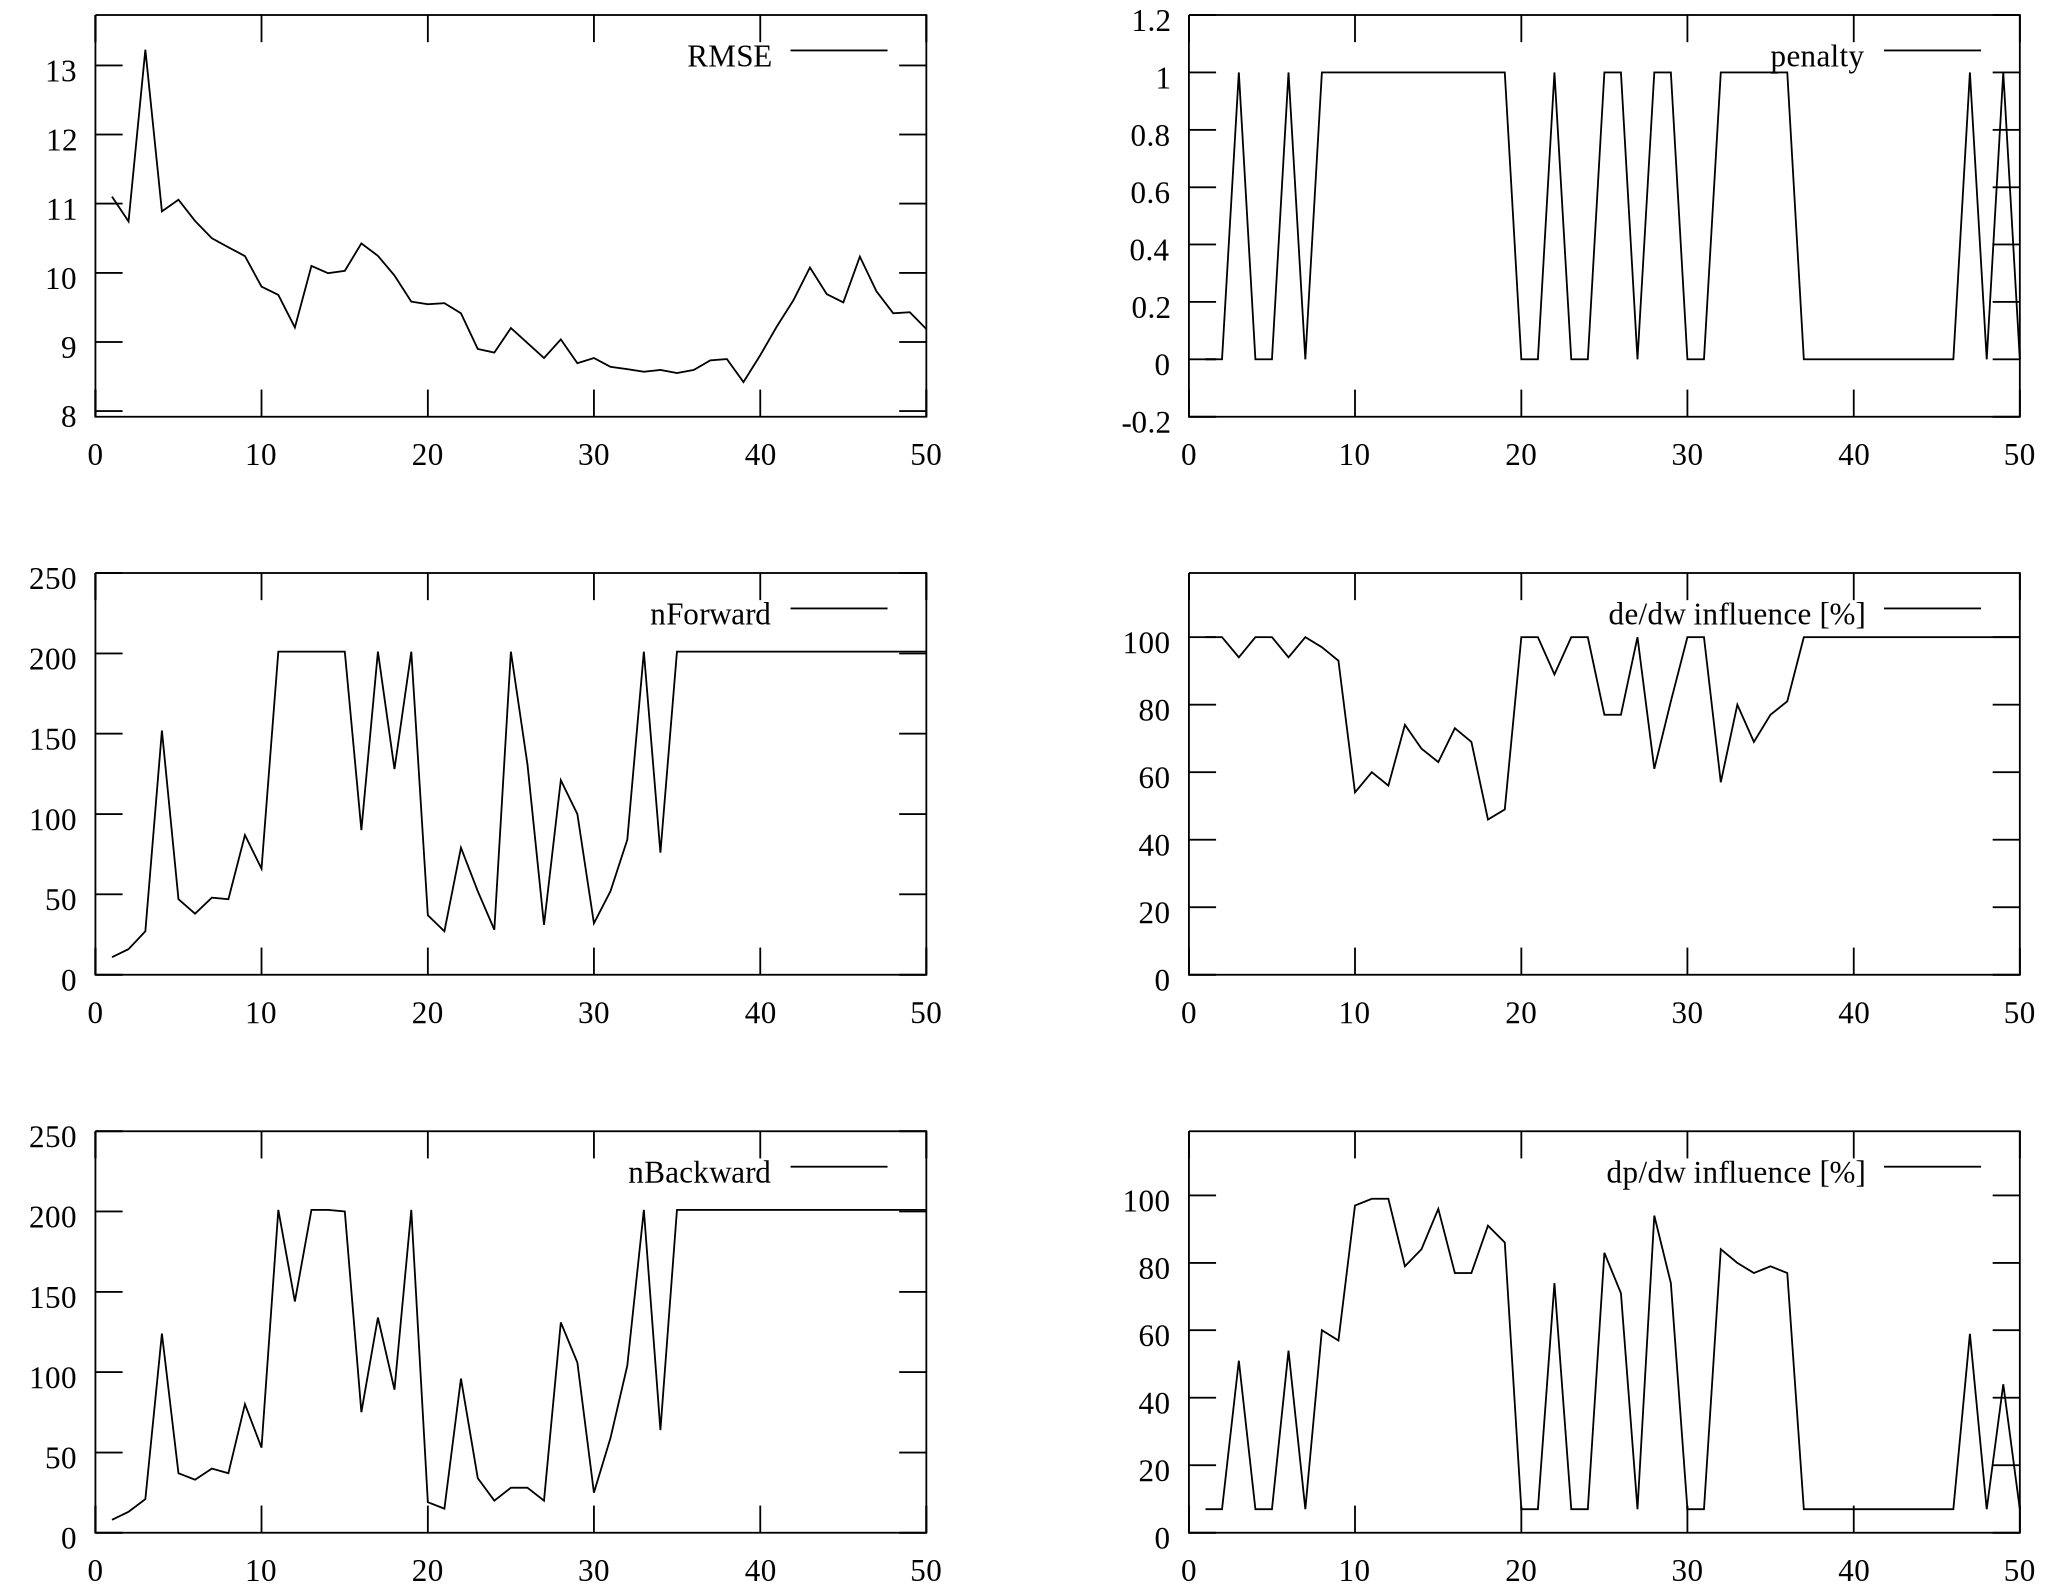
\includegraphics[scale=0.09]{img/gnn1_2}
	\caption{gnn5 performance with $\mu = 0.9$ for 20 graphs}
	\label{fig:gnn5_09}
\end{center}
\end{figure}

A different situation is shown for $\mu = 0.6$. Because of a low $\mu$ value, the penalty was imposed eagerly and was larger than in the previous case (the impact of the $\mu$ value was described in section~\ref{sec:contraction}). It was imposed even when the number of \emph{Forward} steps was below the maximum, that is when $F_{\bm{w}}$ was still a contraction map. Large values of the penalty caused a huge decrease of the $\frac{\partial e}{\partial w}$ term influence, which made any learning impossible.

\begin{figure}[h!]
\begin{center}
	\includegraphics[scale=0.09]{img/gnn1_3}
	\caption{gnn5 performance with $\mu = 0.6$ for 20 graphs}
	\label{fig:gnn5_06}
\end{center}
\end{figure}

\newpage
Another interesting case is presented in Fig.~\ref{fig:gnn5_09_10}: the learning process of gnn5 on 10 graphs with $\mu = 0.9$. It can be observed that even as the number of \emph{Forward} steps reached in peaks the maximum value, the $F_{\bm{w}}$ function remained a contraction map. A large enough $\mu$ prevented the penalty from being imposed, which enabled the GNN model to train both computation units without any disturbance. The result is a monotonously decreasing RMSE slope, which could be previously observed in Fig.~\ref{fig:gnn_multiple}. It can be concluded, that the most important aspect of building a GNN model is to provide an efficient way to make $F_{\bm{w}}$ a contraction map as fast as possible, so as to provide as much time as possible for undisturbed learning.

\newpage
\begin{figure}[h!]
\begin{center}
	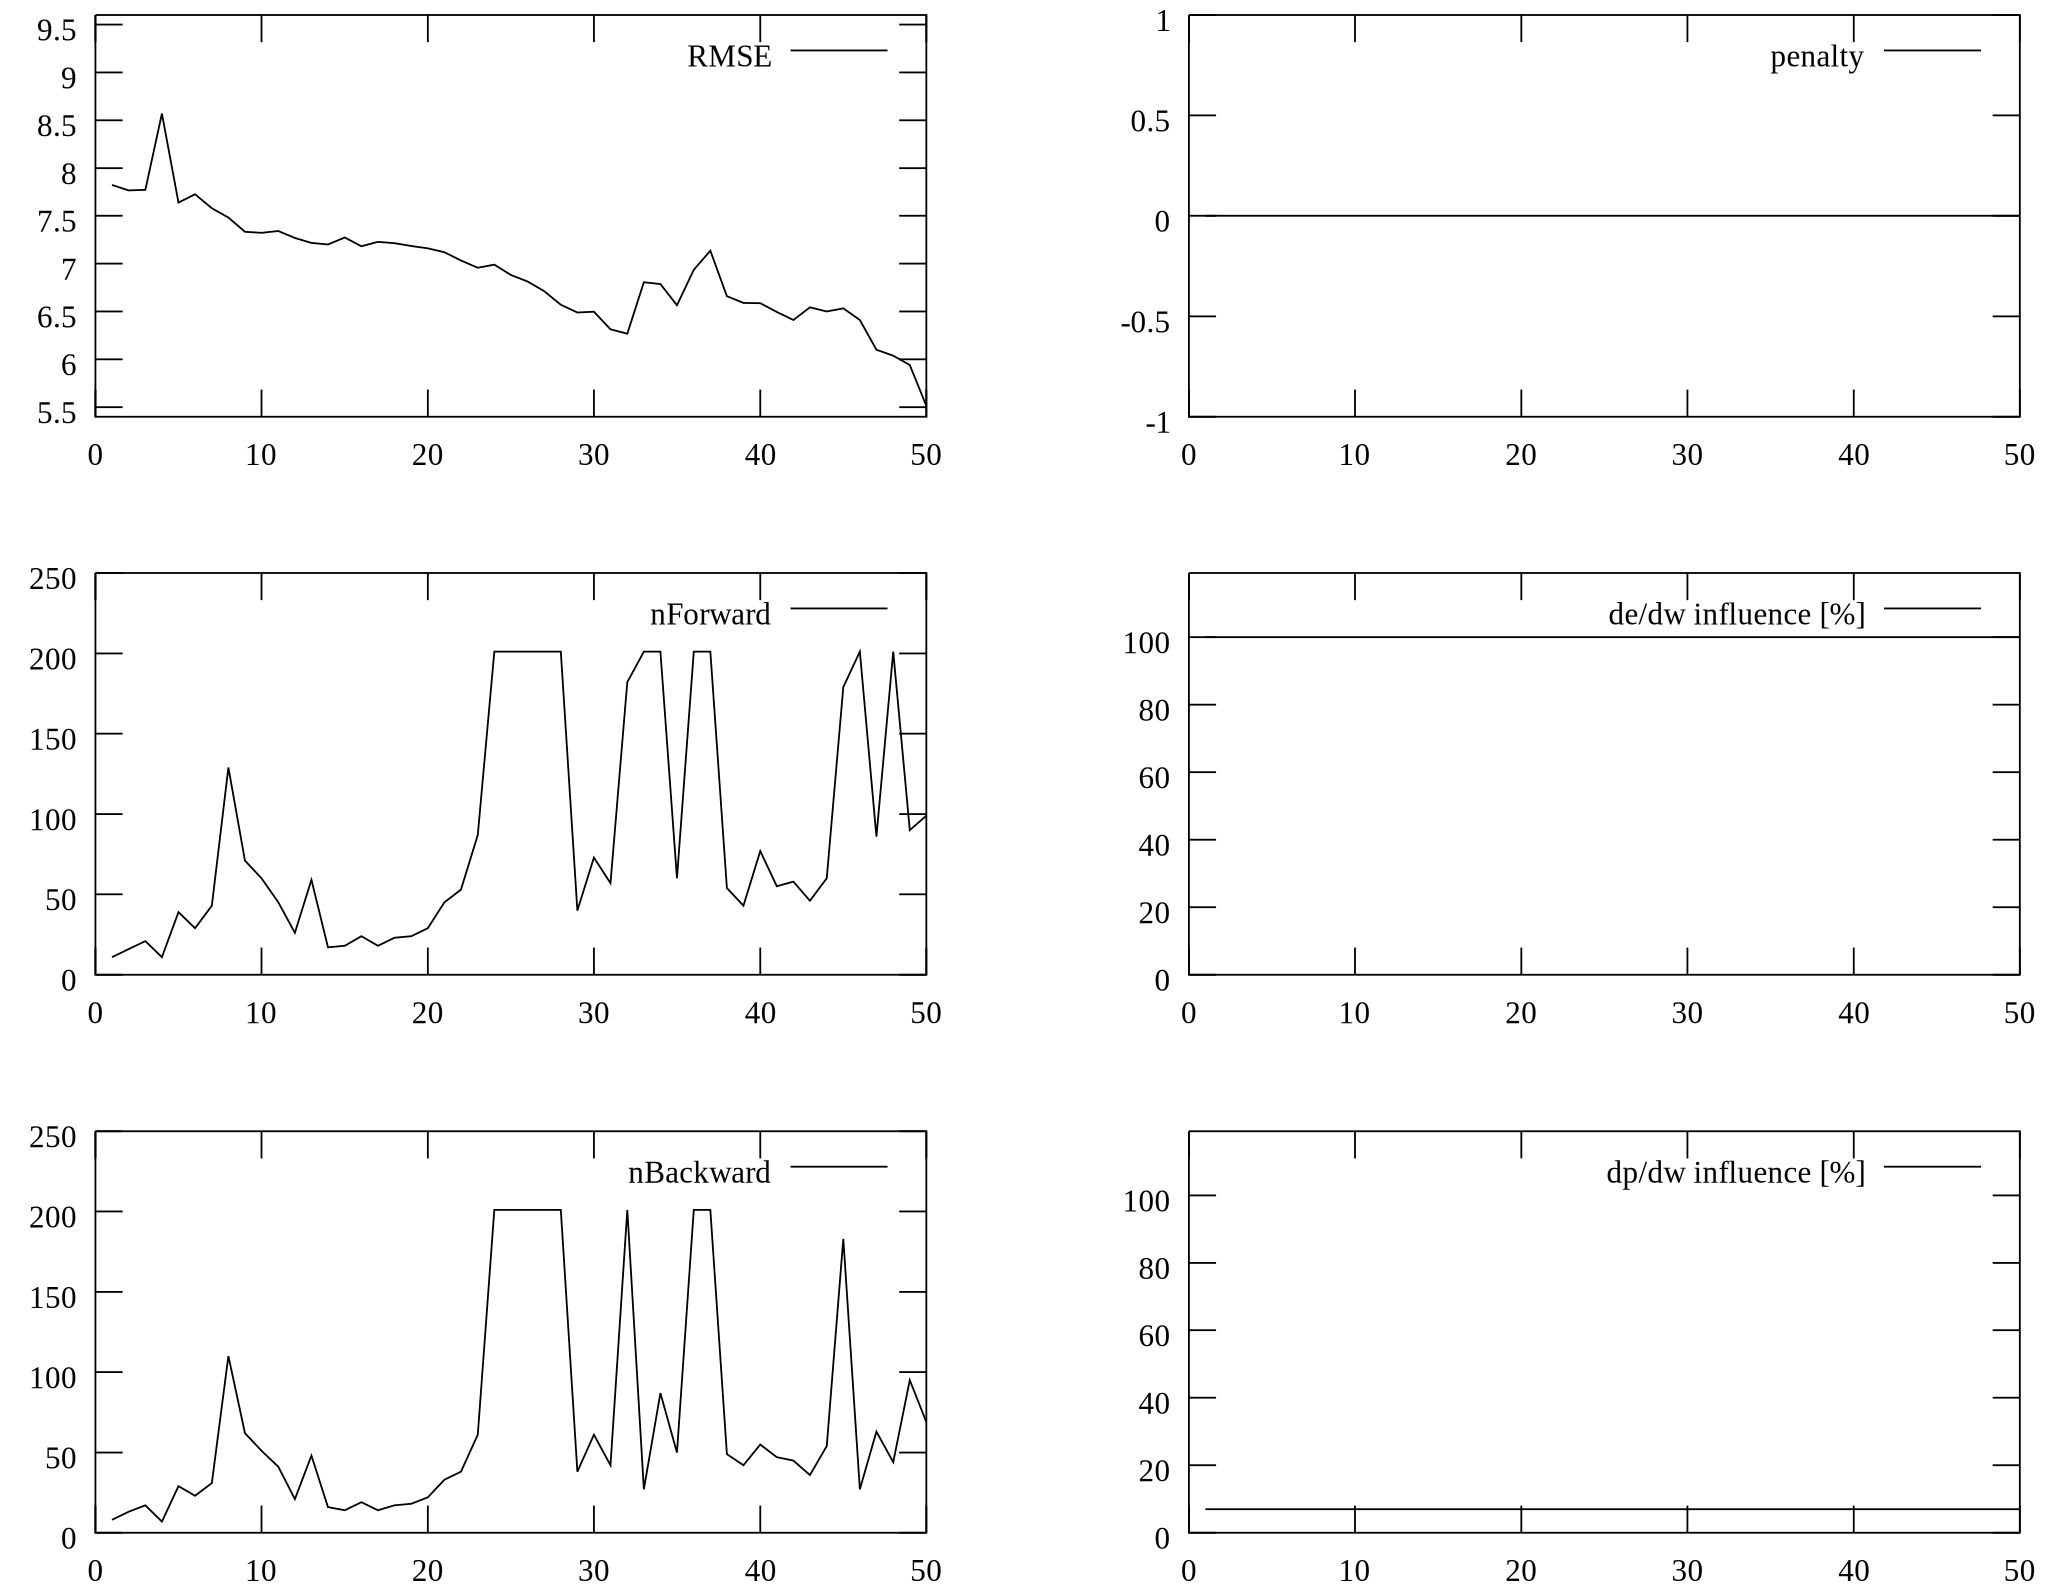
\includegraphics[scale=0.09]{img/gnn5}
	\caption{gnn5 performance with $\mu = 0.9$ for 10 graphs}
	\label{fig:gnn5_09_10}
\end{center}
\end{figure}

\newpage
\section{Cross-validation results}
To compare the performance of the implemented GNN model with a standard FNN, the following subgraph matching experiment was conducted. 5-fold cross-validation was performed on all 100 graphs from the 14-7 dataset. A random GNN was generated. It was trained with a contraction constant $\mu = 0.9$ for 50 iterations for each fold. To provide good FNN results, 10 three-layer FNNs with 20 hidden $tanh$ neurons were evaluated and the one with best mean accuracy was selected. The results are presented in Table~\ref{tab:crossmean} and~\ref{tab:crossstd}. The GNN classifier outperformed the FNN by more than 15\%. This is due to the fact, that the FNN classifier could make predictions only by analyzing node labels, while the GNN classifier exploited correctly the graph topology.

These results can be better understood by analyzing the classified dataset. The 100 processed graphs consisted in total of 1400 nodes. Amongst these nodes, 1031 had node labels matching the subgraph node labels. Amongst these 1031 nodes only 702 actually belonged to the subgraph. Thus, 329 nodes, 23.5\% of all the nodes would probably be classified as false positives by a classifier taking into consideration only node labels. This hypothesis corresponds quite well with the results presented.

\begin{table}[h!]
	\begin{center}
	\begin{tabular}{llll}
	\toprule
	& accuracy & precision & recall \\
	\midrule
	FNN - tr &	75\% &  68\% &  93\% \\
	FNN - tst &	74\% &  68\% &  93\% \\
	GNN - tr &	91\% &  87\% &  97\% \\
	GNN - tst &	91\% &  86\% &  97\% \\
	\bottomrule
	\end{tabular}
	\caption{Mean values on training and test sets}
	\label{tab:crossmean}
	\end{center}
\end{table}

\begin{table}[h!]
	\begin{center}
	\begin{tabular}{llll}
	\toprule
	& accuracy & precision & recall \\
	\midrule
	FNN - tr &	0.68\% &  0.82\% &  1.43\% \\
	FNN - tst &	3.20\% &  2.89\% &  1.85\% \\
	GNN - tr &	1.62\% &  1.71\% &  2.07\% \\
	GNN - tst &	3.06\% &  3.70\% &  1.39\% \\
	\bottomrule
	\end{tabular}
	\caption{Standard deviations on training and test sets}
	\label{tab:crossstd}
	\end{center}
\end{table}


\chapter{Conclusions}
The implementation of the GNN model yielded promising experimental results for structured data and proved that it can exploit properly both node labels and the graph structure. Some changes in the original algorithm, as the maximum number of \emph{Forward} and \emph{Backward} iterations were introduced to assure a more predictable computation time. Conditions under which the model works efficiently were described. An important parameter of the GNN model, determining the training efficiency was identified: the contraction constant $\mu$. The most important conclusions are listed below:
\begin{itemize}
	\item training yields best results when $F_{\bm{w}}$ remains a contraction map,
	\item if $F_{\bm{w}}$ definitely ceases to be a contraction map, there are no training effects,
	\item remaining near the contraction state can still yield good results,
	\item a fixed maximum number of \emph{Forward}/\emph{Backward} iterations can still yield good results,
	\item imposing an unnecessary penalty should be avoided,
	\item too large penalties (a too small $\mu$) should be avoided,
	\item the minimum value of $\mu$ should be tuned to the processed dataset,
	\item the minimum value of $\mu$ can be tuned using a subset of the data.
\end{itemize}


\appendix
%
\chapter{Penalty calculation equations}


\chapter{Using the software\label{chapter:using}}
\noindent The GNN classifier was implemented in GNU Octave 3.6.2 and tested on a x86\_64 PC. The most important functions are:
\begin{itemize}
	\item loadgraph - loads a single graph from .csv files
	\item loadset - loads a set of graphs sharing the same filename prefix
	\item mergegraphs - merge a cellarray of graphs to a single graph
	\item initgnn - initialize a new GNN
	\item traingnn - train GNN using a training graph
	\item classifygnn - classify given graph with a trained GNN
	\item evaluate - evaluate the classification results
	\item crossvalidate - perform cross-validation using an untrained GNN and a set of graphs
\end{itemize}
\noindent Help and usage information for each function can be displayed by typing \emph{help <function\_name>} in the Octave command line.\\



\begin{lstlisting}[style=outcode, language=Matlab, caption=Sample usage session]
g6 = loadset('../data/g6s3n/g6s3', 10);
gm = mergegraphs(g6);
gnn = initgnn(gm, 5, [5 5], 'tansig');
trainedGnn = traingnn(gnn, gm, 20);
outputs = classifygnn(trainedGnn, gm);
stats = evaluate(outputs, gm.expectedOutput);
\end{lstlisting}

\noindent All subgraph matching datasets were created using the \emph{buildgraphs.py} script. Each graph can be viewed as a pdf file by using the \emph{drawgraph.py} script. Each graph is stored as three .csv files, containing node labels, edge labels and expected outputs. A sample graph \emph{'test'} is presented below. Nodes yielding output 2 were marked as black.

\begin{figure}
\begin{floatrow}
\ffigbox[\FBwidth]{	% use the image width
	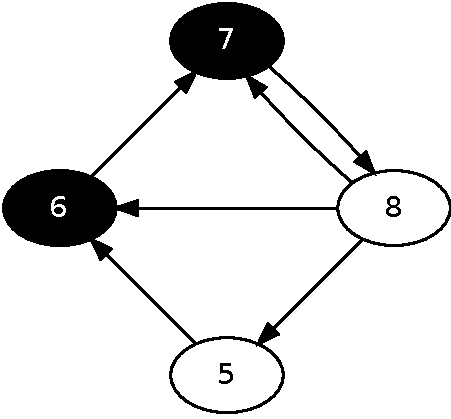
\includegraphics[scale=0.55]{img/test}
}{
\caption{Sample graph}
}
\capbtabbox{
	\begin{tabular}{lll}
	\toprule
	test\_nodes.csv & test\_output.csv & test\_edges.csv \\
	\midrule
	5	&	1	&	1,2,0\\
	6	&	2	&	2,3,0\\
	7	&	2	&	3,4,0\\
	8	&	1	&	4,1,0\\
		&		&	4,2,0\\
		&		&	4,3,0\\
	\bottomrule
	\end{tabular}
}{
\caption{Sample graph data}%
}
\end{floatrow}
\end{figure}

%
\chapter{Listings\label{chap:code}}

\lstinputlisting[style=outcode, language=Matlab, breaklines=true, caption=Main training function]{../srcf/traingnn.m}

\newpage
\lstinputlisting[style=outcode, language=Matlab, breaklines=true, caption=Forward function]{../src/forward.m}
\lstinputlisting[style=outcode, language=Matlab, breaklines=true, caption=Transition function]{../srcf/transition.m}
\lstinputlisting[style=outcode, language=Matlab, caption=State convergence check]{../srcf/stablestate.m}

\newpage
\lstinputlisting[style=outcode, language=Matlab, breaklines=true, caption=Backward function]{../srcf/backward.m}
\newpage
\lstinputlisting[style=outcode, language=Matlab, breaklines=true, caption=Matrix A calculation]{../srcf/calculatea.m}
\newpage
\lstinputlisting[style=outcode, language=Matlab, breaklines=true, caption=Matrix b calculation]{../srcf/calculateb.m}

\newpage
\lstinputlisting[style=outcode, language=Matlab, breaklines=true, caption=Penalty derivative calculation]{../srcf/penaltyderivative.m}

\newpage
\lstinputlisting[style=outcode, language=Matlab, breaklines=true, caption=RPROP weights update]{../srcf/rpropupdate.m}


%\listoftables
\listoffigures

%\lstlistoflistings
%\addcontentsline{toc}{chapter}{List of Listings}

%\nocite{*}
%\bibliographystyle{plplain}
\bibliographystyle{ieeetr}
%\bibliographystylebk{plplain}
%\bibliographystylest{plplain}
%\bibliographystyledoc{plplain}
% \bibliographystyleweb{plplain}
%\bibliographybk{BIB/books}
%\bibliographyst{BIB/books}
%\bibliographydoc{BIB/books}
% \bibliographyweb{BIB/books}

\bibliography{bib/gnn}

\end{document}

% ex: set tabstop=4 shiftwidth=4 softtabstop=4 noexpandtab fileformat=unix filetype=tex spelllang=pl,en spell:

